\documentclass[10pt,aspectratio=43,xcolor=x11names,t]{beamer}%aspectratio=169,


%\usepackage[space=false]{ctex}
\usepackage{fontspec,xunicode,xltxtra}
\usepackage{hyperref}	
\usepackage{booktabs}	
\usepackage{mathrsfs,amssymb,amsfonts,amsmath,bm}	%Math packages
\usepackage[all]{xy}
\usepackage{dsfont}     %double line number
\usepackage{color}
\usepackage{xcolor}
\usepackage{graphicx,psfrag}
\usepackage{epsfig}
\usepackage{array, booktabs}
\usepackage{graphicx}
\usepackage{caption}
\usepackage{slashed}	%Dirac Operator
\usepackage{tikz}
	\usetikzlibrary{calc}
	\usetikzlibrary{decorations.markings}
	\usetikzlibrary{arrows}
\usepackage{extarrows}
\usepackage[export]{adjustbox}
\usepackage{lipsum}
\usepackage[many]{tcolorbox} % see https://tex.stackexchange.com/questions/135331/how-to-draw-a-big-red-cross-through-large-parts-of-a-text
\usepackage{multicol} % see https://tex.stackexchange.com/questions/194426/split-itemize-into-multiple-columns

\newtcolorbox{cross}{blank,breakable,parbox=false,
  overlay={\draw[red,line width=5pt] (interior.south west)--(interior.north east);
    \draw[red,line width=5pt] (interior.north west)--(interior.south east);}}


\def\Re{\mathop{\mathcal{R}e}}
\def\Im{\mathop{\mathcal{I}m}}
\def\arrow{\tikz[scale=0.1,baseline=.1ex]{
	\draw[fill=black,rotate=-90] (-0.7,0)--(0,2)--(0.7,0);}
	}

\def\cross{\tikz[scale=0.1,baseline=.1ex]{
	\draw[thick,rotate=45] (-1,0)--(1,0);
	\draw[thick,rotate=45] (0,-1)--(0,1);}
	}

\newcommand*\dd{\mathop{}\!\mathrm{d}}
\newcommand*\ddd[1]{\mathop{}\!\mathrm{d^#1}}
\def\Re{\mathop{\mathcal{R}e}}					%Real part
\def\Im{\mathop{\mathcal{I}m}}					%imaginary part
\def\imp{\text{imp}}

\mode <presentation>
%\usetheme{Madrid}%% default Warsaw [secheader]
%\usetheme{Warsaw}%% tested by hxd
\usetheme{CambridgeUS}
\usecolortheme{beaver} %% changed by hxd, red style
\beamersetaveragebackground{black!10} % gray scale background

\setbeamercovered{transparent}
%\setbeamertemplate{navigation symbols}{}

\usefonttheme{professionalfonts}
\useinnertheme{circles}%{rectangles}
\setbeamertemplate{itemize item}{$\circledast$}% design the item bullet %\circledast  %\checkmark


\DeclareCaptionFont{blue}{\color{orange}}%LightSteelBlue3

\newcommand{\foo}{\color{blue}\makebox[0pt]{\textbullet}\hskip-0.5pt\vrule width 1pt\hspace{\labelsep}}%LightSteelBlue3

\hypersetup{pdfpagemode=FullScreen} % makes your presentation go automatically to full screen
%\setcounter{tocdepth}{1} % depth of table of contents

\defbeamertemplate{title page}{English}{ % English version of title page, use by \setbeamertemplate{title page}[Chinese/English]
	%\vbox{}
	\vfill
	\begin{center}
		
\includegraphics[height=2.0cm]{BC-Eagle.svg}
		\vskip1em\par%
		\begin{beamercolorbox}[sep=8pt,center,shadow=true,rounded=true]{title}
			\usebeamerfont{title}\inserttitle\par%
			\ifx\insertsubtitle\@empty%
			\else%
				\vskip0.25em%
				{\usebeamerfont{subtitle}\usebeamercolor[fg]{subtitle}\insertsubtitle\par}%
			\fi%
		\end{beamercolorbox}%
		%\vskip1em\par
		%\begin{beamercolorbox}[sep=8pt,center]{author}
		%	\usebeamerfont{author}%\insertauthor
		%	{
		%	    \begin{tabular}{cc}
		%	    Respondant: &\insertauthor\\ %答辩人:
		%	    Supervisor: &\advisor %导\quad 师:
		%	    \end{tabular}
		%	}
		\end{beamercolorbox}
		\begin{beamercolorbox}[sep=6pt,center]{institute} %sep means separationb between beamercolorboxes
			\usebeamerfont{institute}\insertinstitute
		\end{beamercolorbox}
		\begin{beamercolorbox}[sep=6pt,center]{date}
			\usebeamerfont{date}\insertdate
		\end{beamercolorbox}\vskip0.5em
		%{\usebeamercolor[fg]{titlegraphic}\inserttitlegraphic\par}
	\end{center}
	\vfill
}

%\setbeamertemplate{section in toc}[ball,hideothersubsections]
%\setbeamertemplate{subsection in toc}[subsections numbered]


\setbeamertemplate{footline}{% change the ratio of each colorbox, cf. https://tex.stackexchange.com/questions/315580/how-to-adjust-width-of-footnotes-in-beamer-cambridgeus-theme/315587
	\leavevmode%
	\hbox{%
		\begin{beamercolorbox}[wd=.25\paperwidth,ht=2.25ex,dp=1ex,center]{author in head/foot}%
			\usebeamerfont{author in head/foot}\insertshortauthor\expandafter~~(\insertshortinstitute)
		\end{beamercolorbox}%
		\begin{beamercolorbox}[wd=.45\paperwidth,ht=2.25ex,dp=1ex,center]{title in head/foot}%
			\usebeamerfont{title in head/foot}\insertshorttitle
		\end{beamercolorbox}%
		\begin{beamercolorbox}[wd=.3\paperwidth,ht=2.25ex,dp=1ex,right]{date in head/foot}%
			\usebeamerfont{date in head/foot}\insertshortdate{}\hspace*{2em}
			\insertframenumber{} / \inserttotalframenumber\hspace*{2ex} 
		\end{beamercolorbox}
	}%
	\vskip0pt%
}

%%%%%%%%% set environments like block's color %%%%%%%%%%%
	\setbeamercolor{block title}{use=structure,fg=structure.fg,bg=structure.fg!20!bg}
	\setbeamercolor{block body}{parent=normal text,use=block title,bg=block title.bg!50!bg}

	\setbeamercolor{block title example}{use=example text,fg=example text.fg,bg=example text.fg!20!bg}
	\setbeamercolor{block body example}{parent=normal text,use=block title example,bg=block title example.bg!50!bg}

	\newenvironment<>{redblock}[1]{%
		\setbeamercolor{block title}{fg=white,bg=red!70!pink}%
		\begin{block}#2{#1}}{\end{block}
	}
	\newenvironment<>{greenblock}[1]{%
		\setbeamercolor{block title}{fg=white,bg=green!70!blue}%
		\begin{block}#2{#1}}{\end{block}
	}

	\addtobeamertemplate{proof begin}{%
		\setbeamercolor{block title}{fg=black,bg=red!50!white}
		\setbeamercolor{block body}{fg=red, bg=red!30!white}
	}{}

	\BeforeBeginEnvironment{theorem}{
		\setbeamercolor{block title}{fg=black,bg=orange!50!white}
		\setbeamercolor{block body}{fg=orange, bg=orange!30!white}
	}
	\AfterEndEnvironment{theorem}{
		\setbeamercolor{block title}{use=structure,fg=structure.fg,bg=structure.fg!20!bg}
		\setbeamercolor{block body}{parent=normal text,use=block title,bg=block title.bg!50!bg, fg=black}
	}

\begin{document}

\title[Theory of Hydrodynamic Transport]{Theory of Hydrodynamic Transport:\\Past and Future}
\subtitle{Research Proposal Examination}
\author[Xiaodong Hu]{Xiaodong Hu\\[1em]Advisor: Ying Ran\\ Committee Member: Xiao Chen, Fazel Tafti}
%\def\advisor{Prof. Guo-Zhu Liu$^{1}$\quad Prof. Ying-Hai Wu$^2$}
\institute[BC]{Boston College}



\date{April 30, 2020}

%\begin{minipage}{6in}
%\centering
%\raisebox{-0.5\height}{
\includegraphics[width=1in]{Princeton.pdf}}
%\hspace*{.2in}
%\raisebox{-0.5\height}{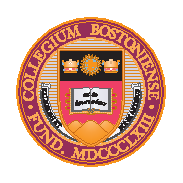
\includegraphics[width=0.5in]{BC-color.eps}}
%\end{minipage}
\titlegraphic{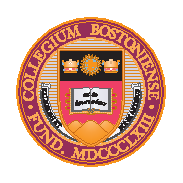
\includegraphics[height=0.5in]{BC-color.eps}}

\begin{frame}%[plain] % without section heads
	\titlepage
\end{frame}


\AtBeginSubsection[]{% add a frame of current position before every section
	\frame{
		\setcounter{tocdepth}{2}
		\frametitle{Contents}
		\tableofcontents[
			currentsection,currentsubsection
		]
	}
}

\begin{frame}
	\frametitle{Outline}
	\tableofcontents
\end{frame}

%%%%%%%%%%%%%%%%%%%%%%%%%%%%%%%%%%%%%%%%%%%%%%%%%%%%%%%%%%%%%%%%%%%%%%%%%%%%%%%

\section{Motivation}

		\begin{frame}\frametitle{Complexity of Condensed Matter}
			The fundamental Hamiltonian of condensed matter incorperates many parts
			\begin{equation*}
				H=H_{\text{el}}+H_{\text{ph}}+H_{\text{imp}}+{\color{red}H_{\text{el-el}}}+{\color{red}H_{\text{el-ph}}}+{\color{red}H_{\text{el-imp}}}+\cdots.
			\end{equation*}
			We already have full understanding of the system with \textbf{weakly-interacting quasiparticles}, like Fermi liquid.\pause\\[1em]
			But for \textbf{strongly-correlated} systems, or systems \textbf{without} well-defined quasiparticle description,
			\begin{itemize}
				\item Theoretically, all perturbative techniques become invalid;
				\item Numerically, 
				\begin{itemize}
					\item Exact diagnalization is limited by the exponential grow of the dimension of many-body Hilbert space;
					\item QMC is known to fail due to fermion sign problem;
					\item DMRG or Tensor Network are still under development for $d>2$;
					\item $\cdots$
				\end{itemize}
			\end{itemize}
		\end{frame}

		\begin{frame}\frametitle{More is Different}
			\begin{columns}
				\begin{column}{0.45\textwidth}
					\begin{figure}[!htp]
						\centering
						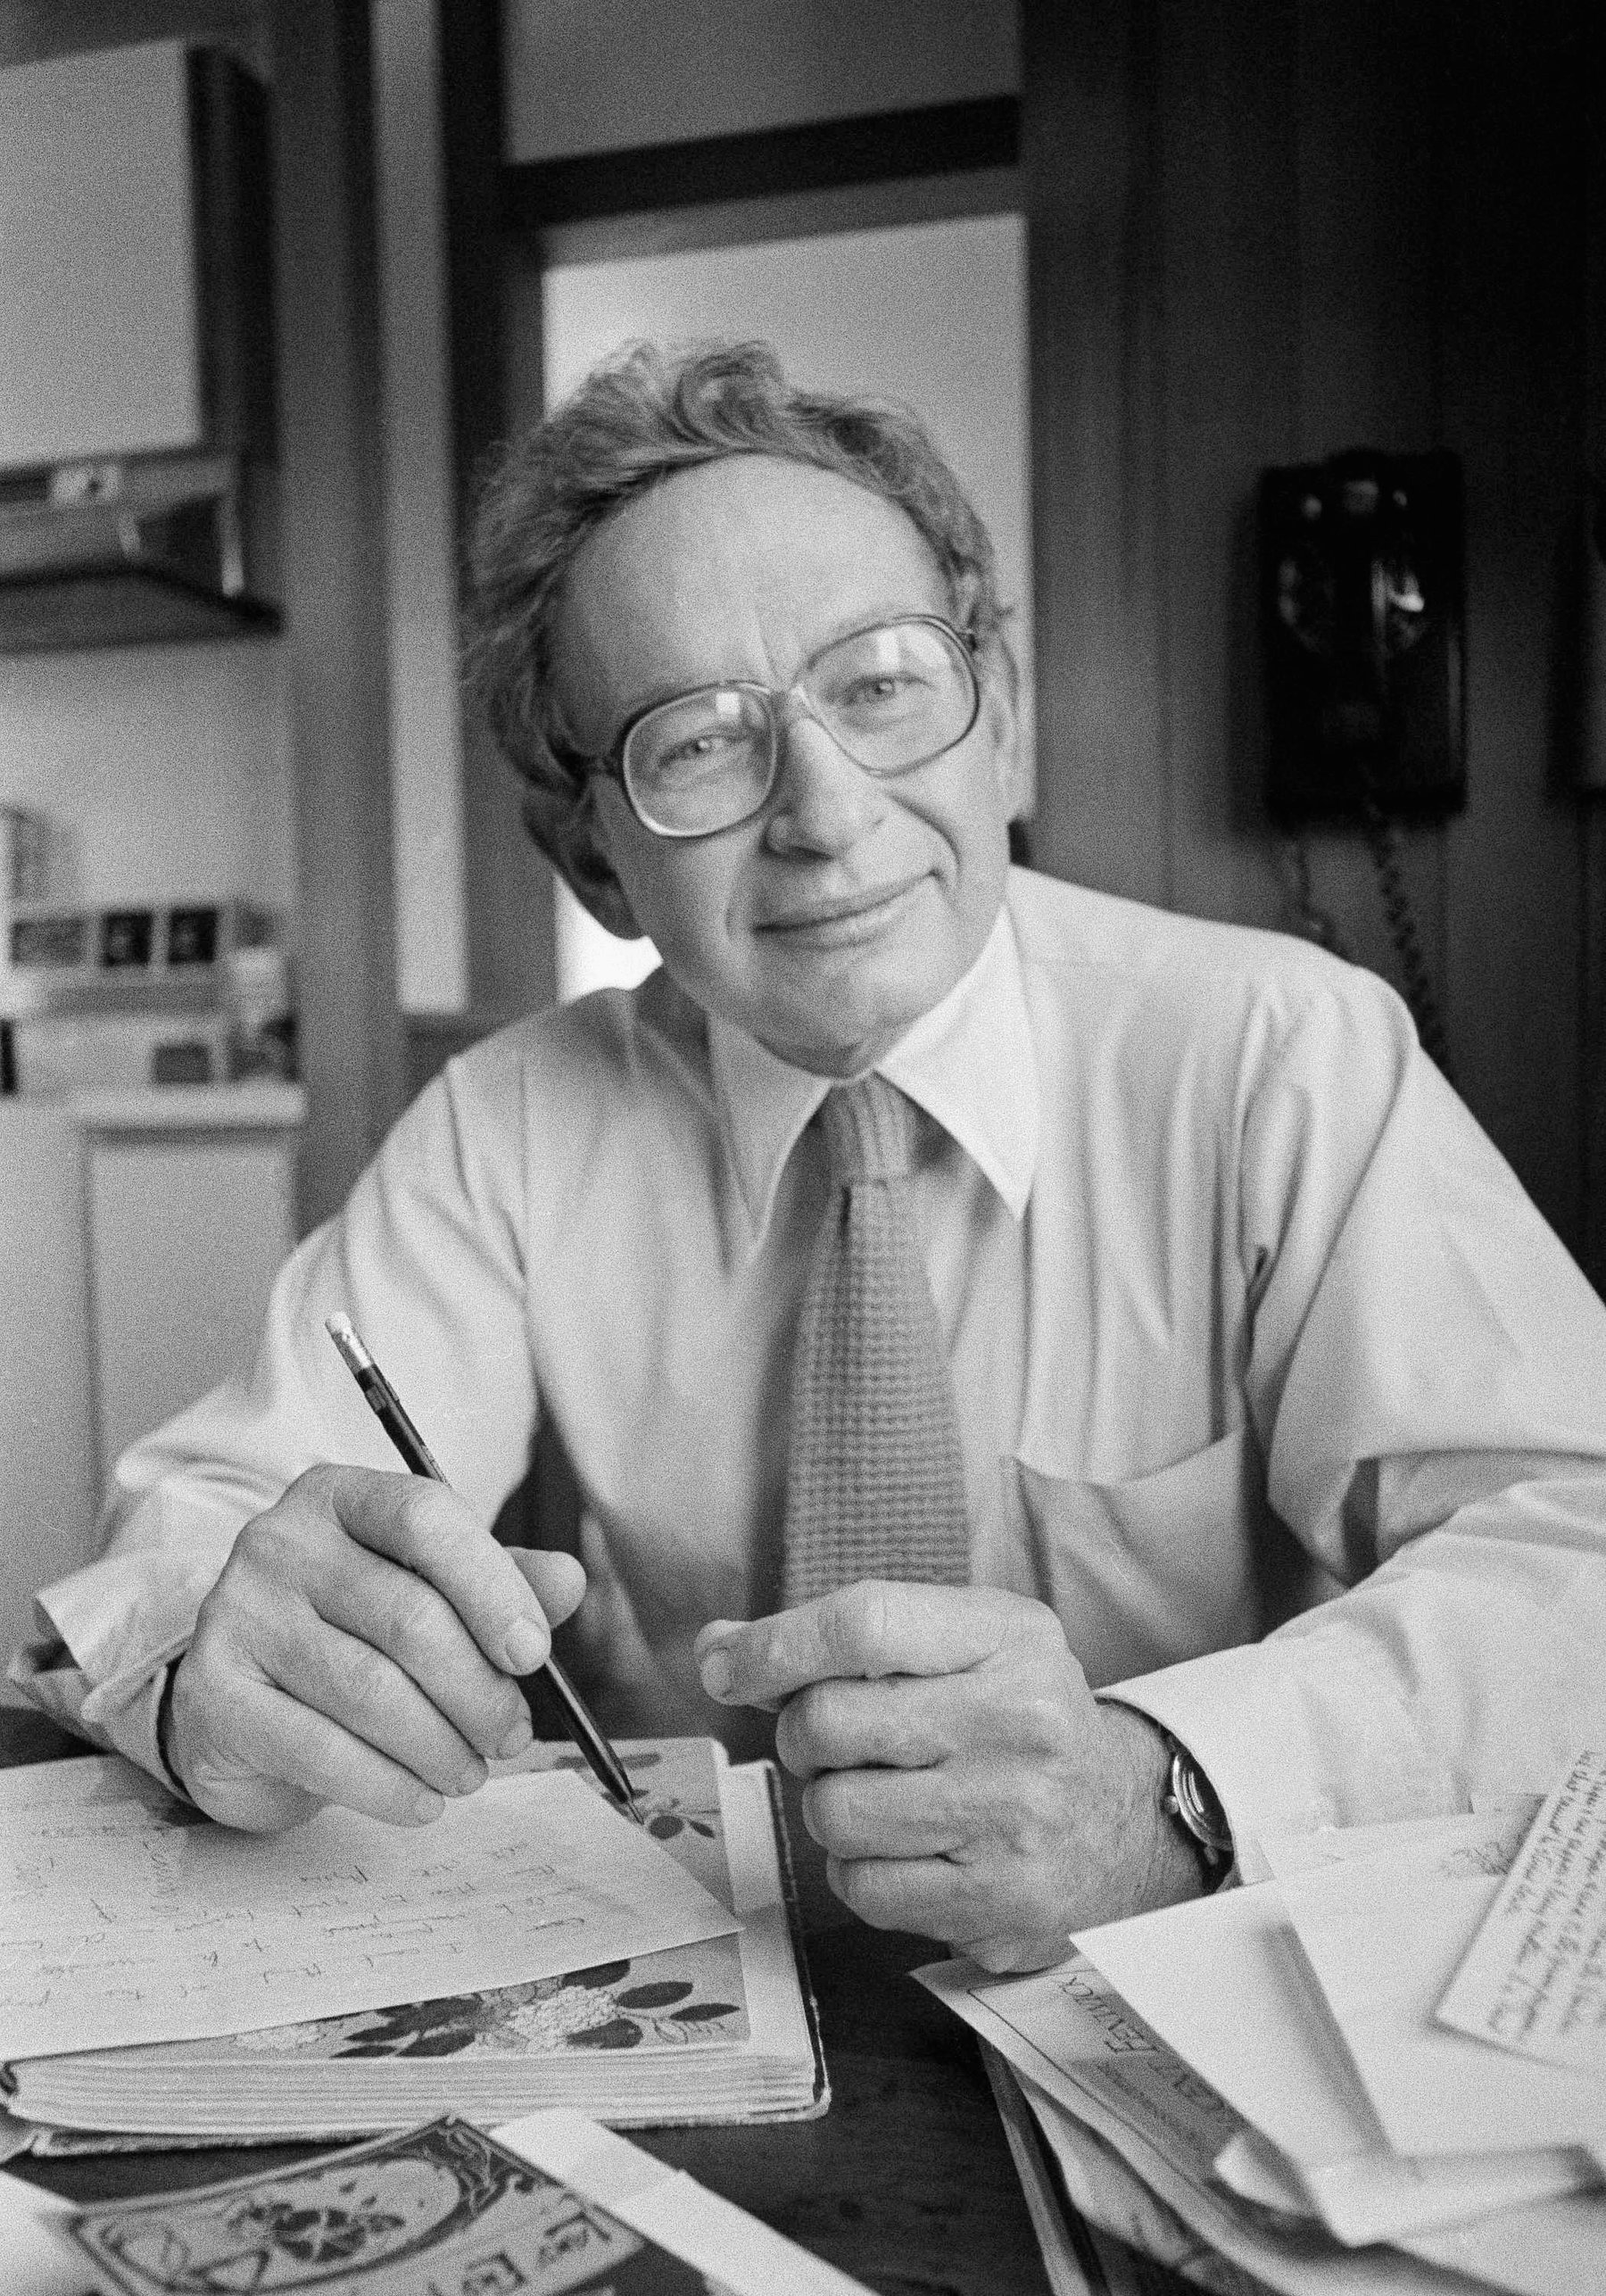
\includegraphics[scale=0.3]{Anderson.jpg}
					\end{figure}
				\end{column}
				\begin{column}{0.5\textwidth}
					\begin{block}{``More is Different''}
						``The behavior of large and complex aggregates of elementary particles, it turns out, is not to be understood in terms of a simple extrapolation of the properties of a few particles.\\Instead, \textbf{\color{red}at each level of complexity entirely new properties appear}, and the understanding of the new behaviors requires research which I think is as fundamental in its nature as any other.''
					\end{block}
					\only<2->{
						\begin{redblock}{Question}
							How to grasp the correct physics without perturbative RG?
						\end{redblock}
					}
				\end{column}				
			\end{columns}
		\end{frame}		

\iffalse		
		\begin{frame}\frametitle{Transport Experiments}
			Experimentally, however, Regardless of the diverse preparation of samples and exclusion of irrelevant factors, there is essentially NO distinguishment for experimentalists to measure a weakly-interacting system or a strongly-correlated system, particularly for transport measurement.
		\end{frame}
\fi

		\begin{frame}\frametitle{Traditional Hydrodynamics}
			\begin{equation*}
				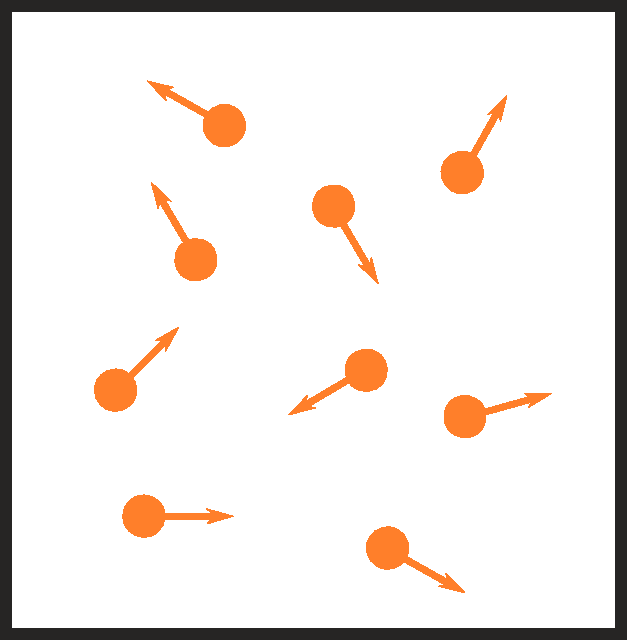
\includegraphics[valign=c,scale=0.3]{gas.pdf}\implies
				\begin{array}{c}
					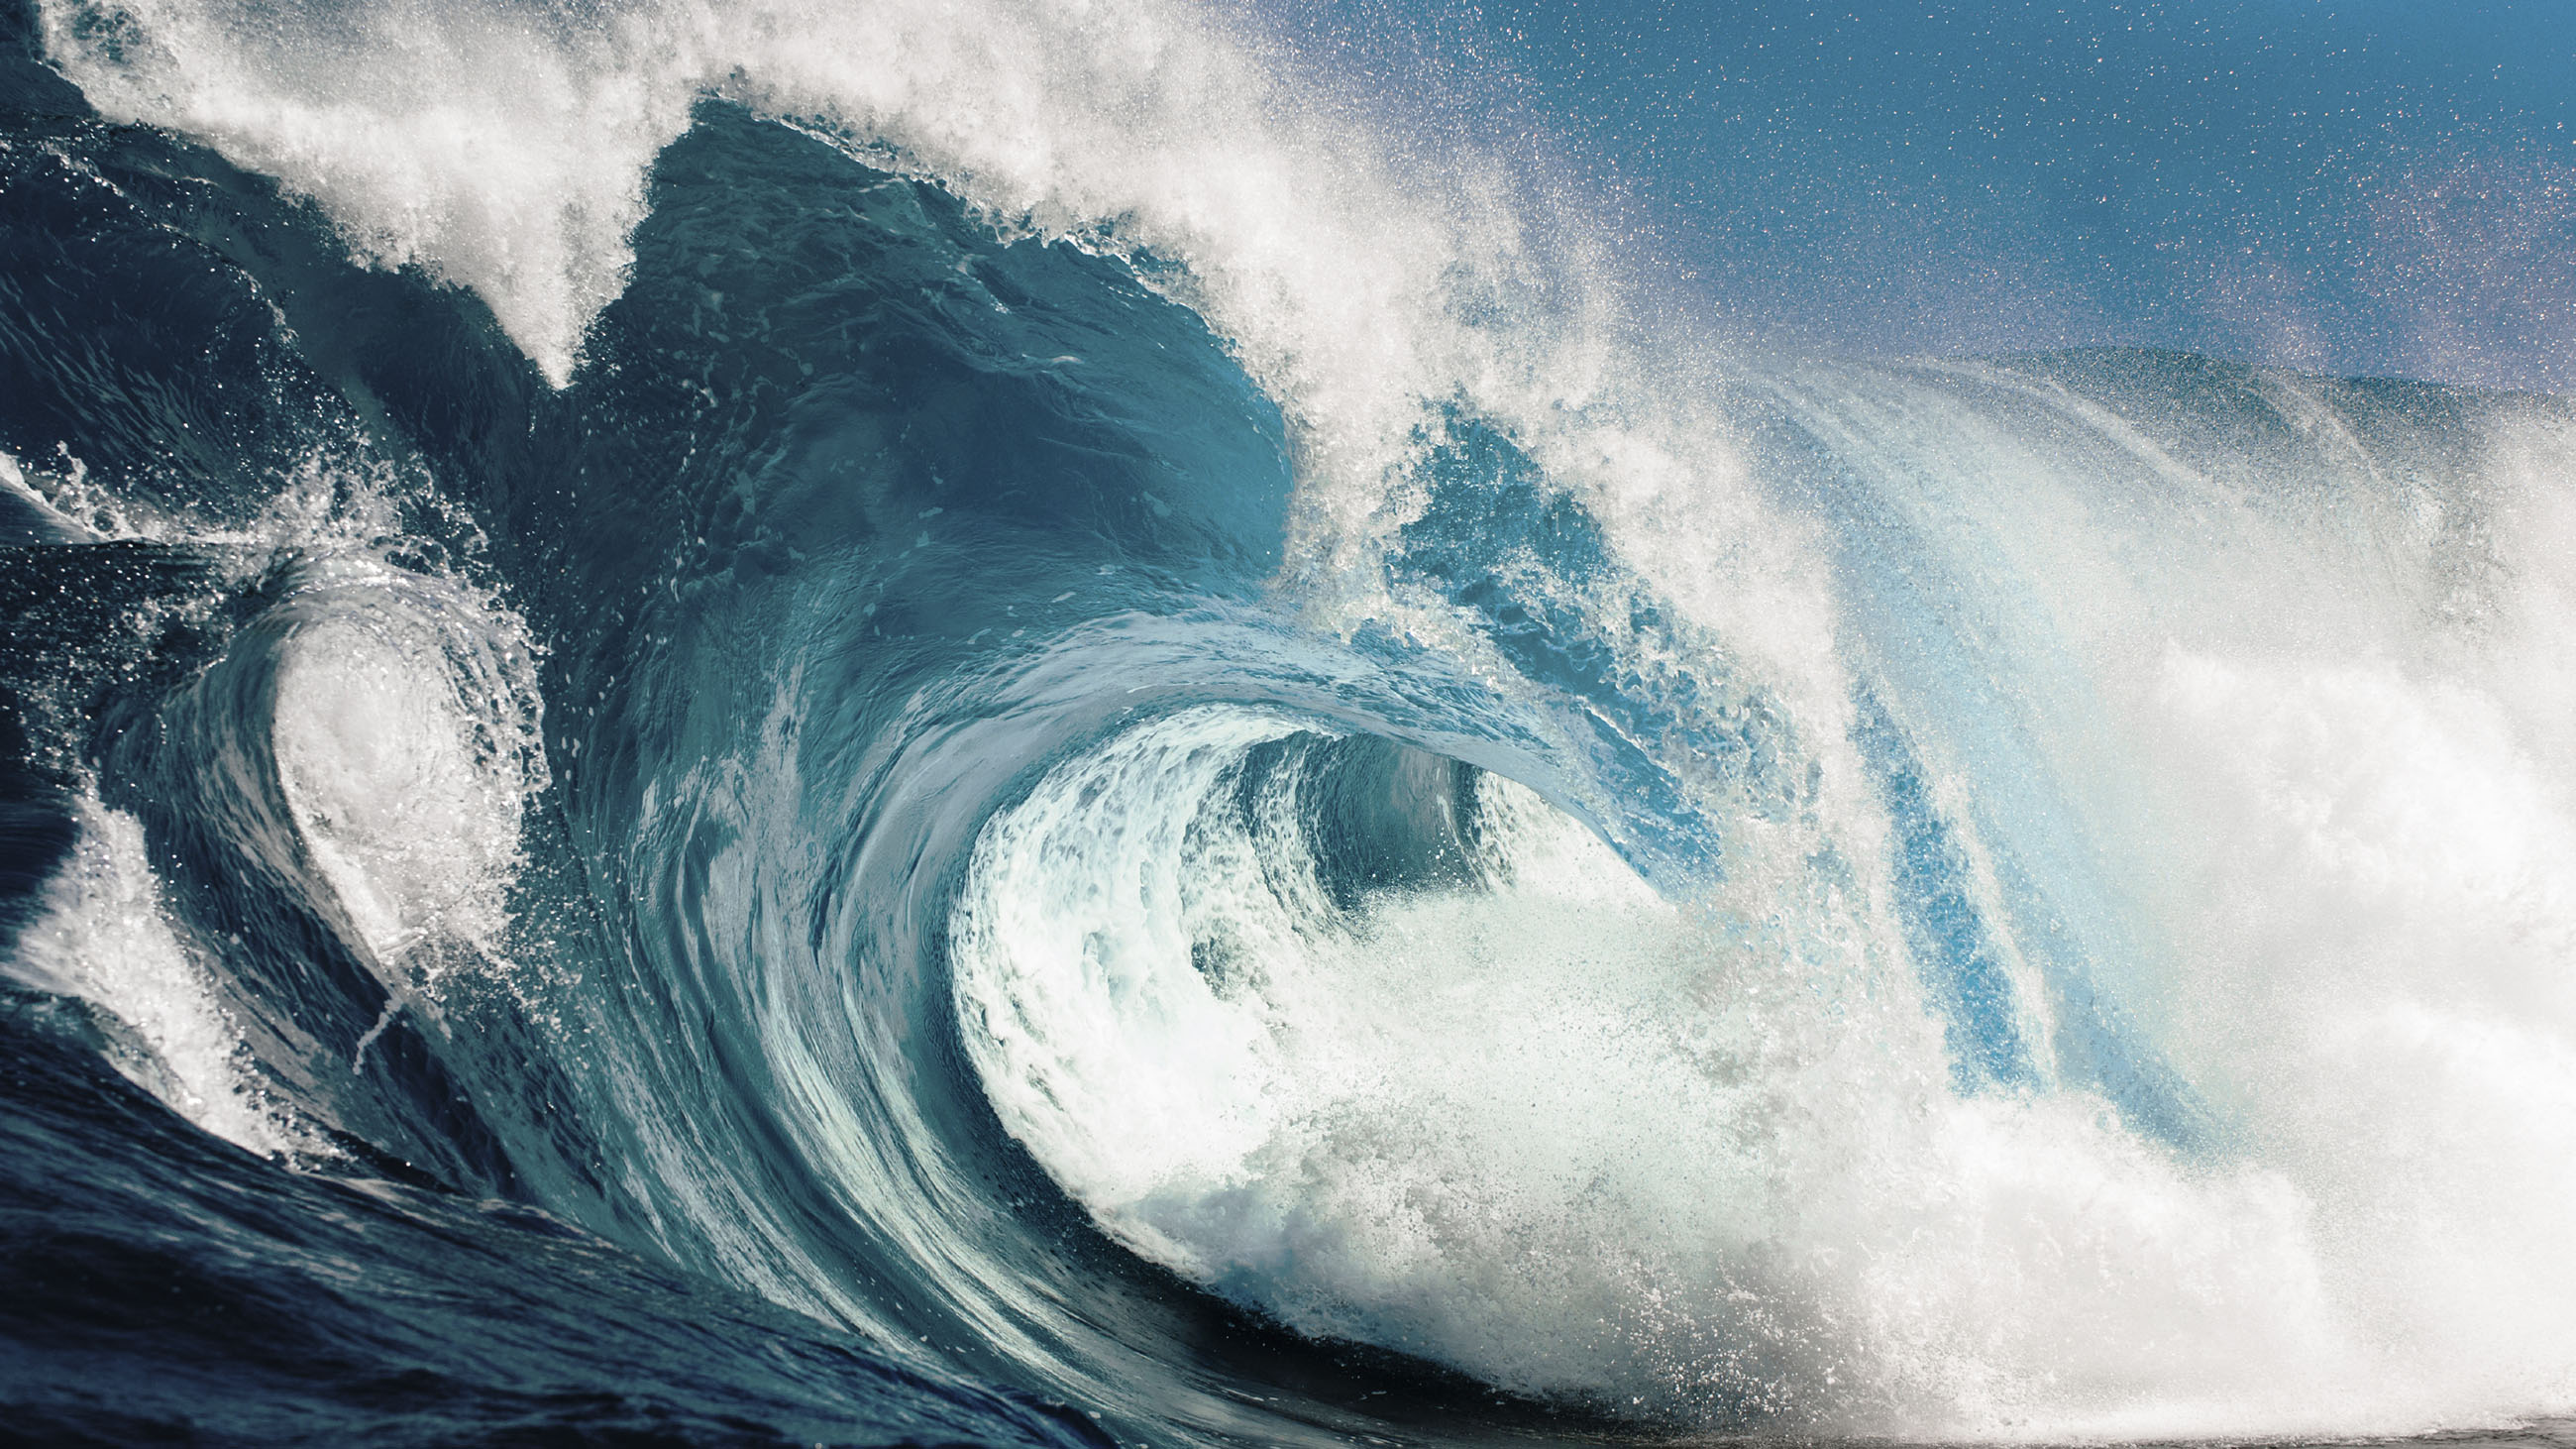
\includegraphics[valign=c,scale=0.2]{ocean.jpg}\\[1em]
					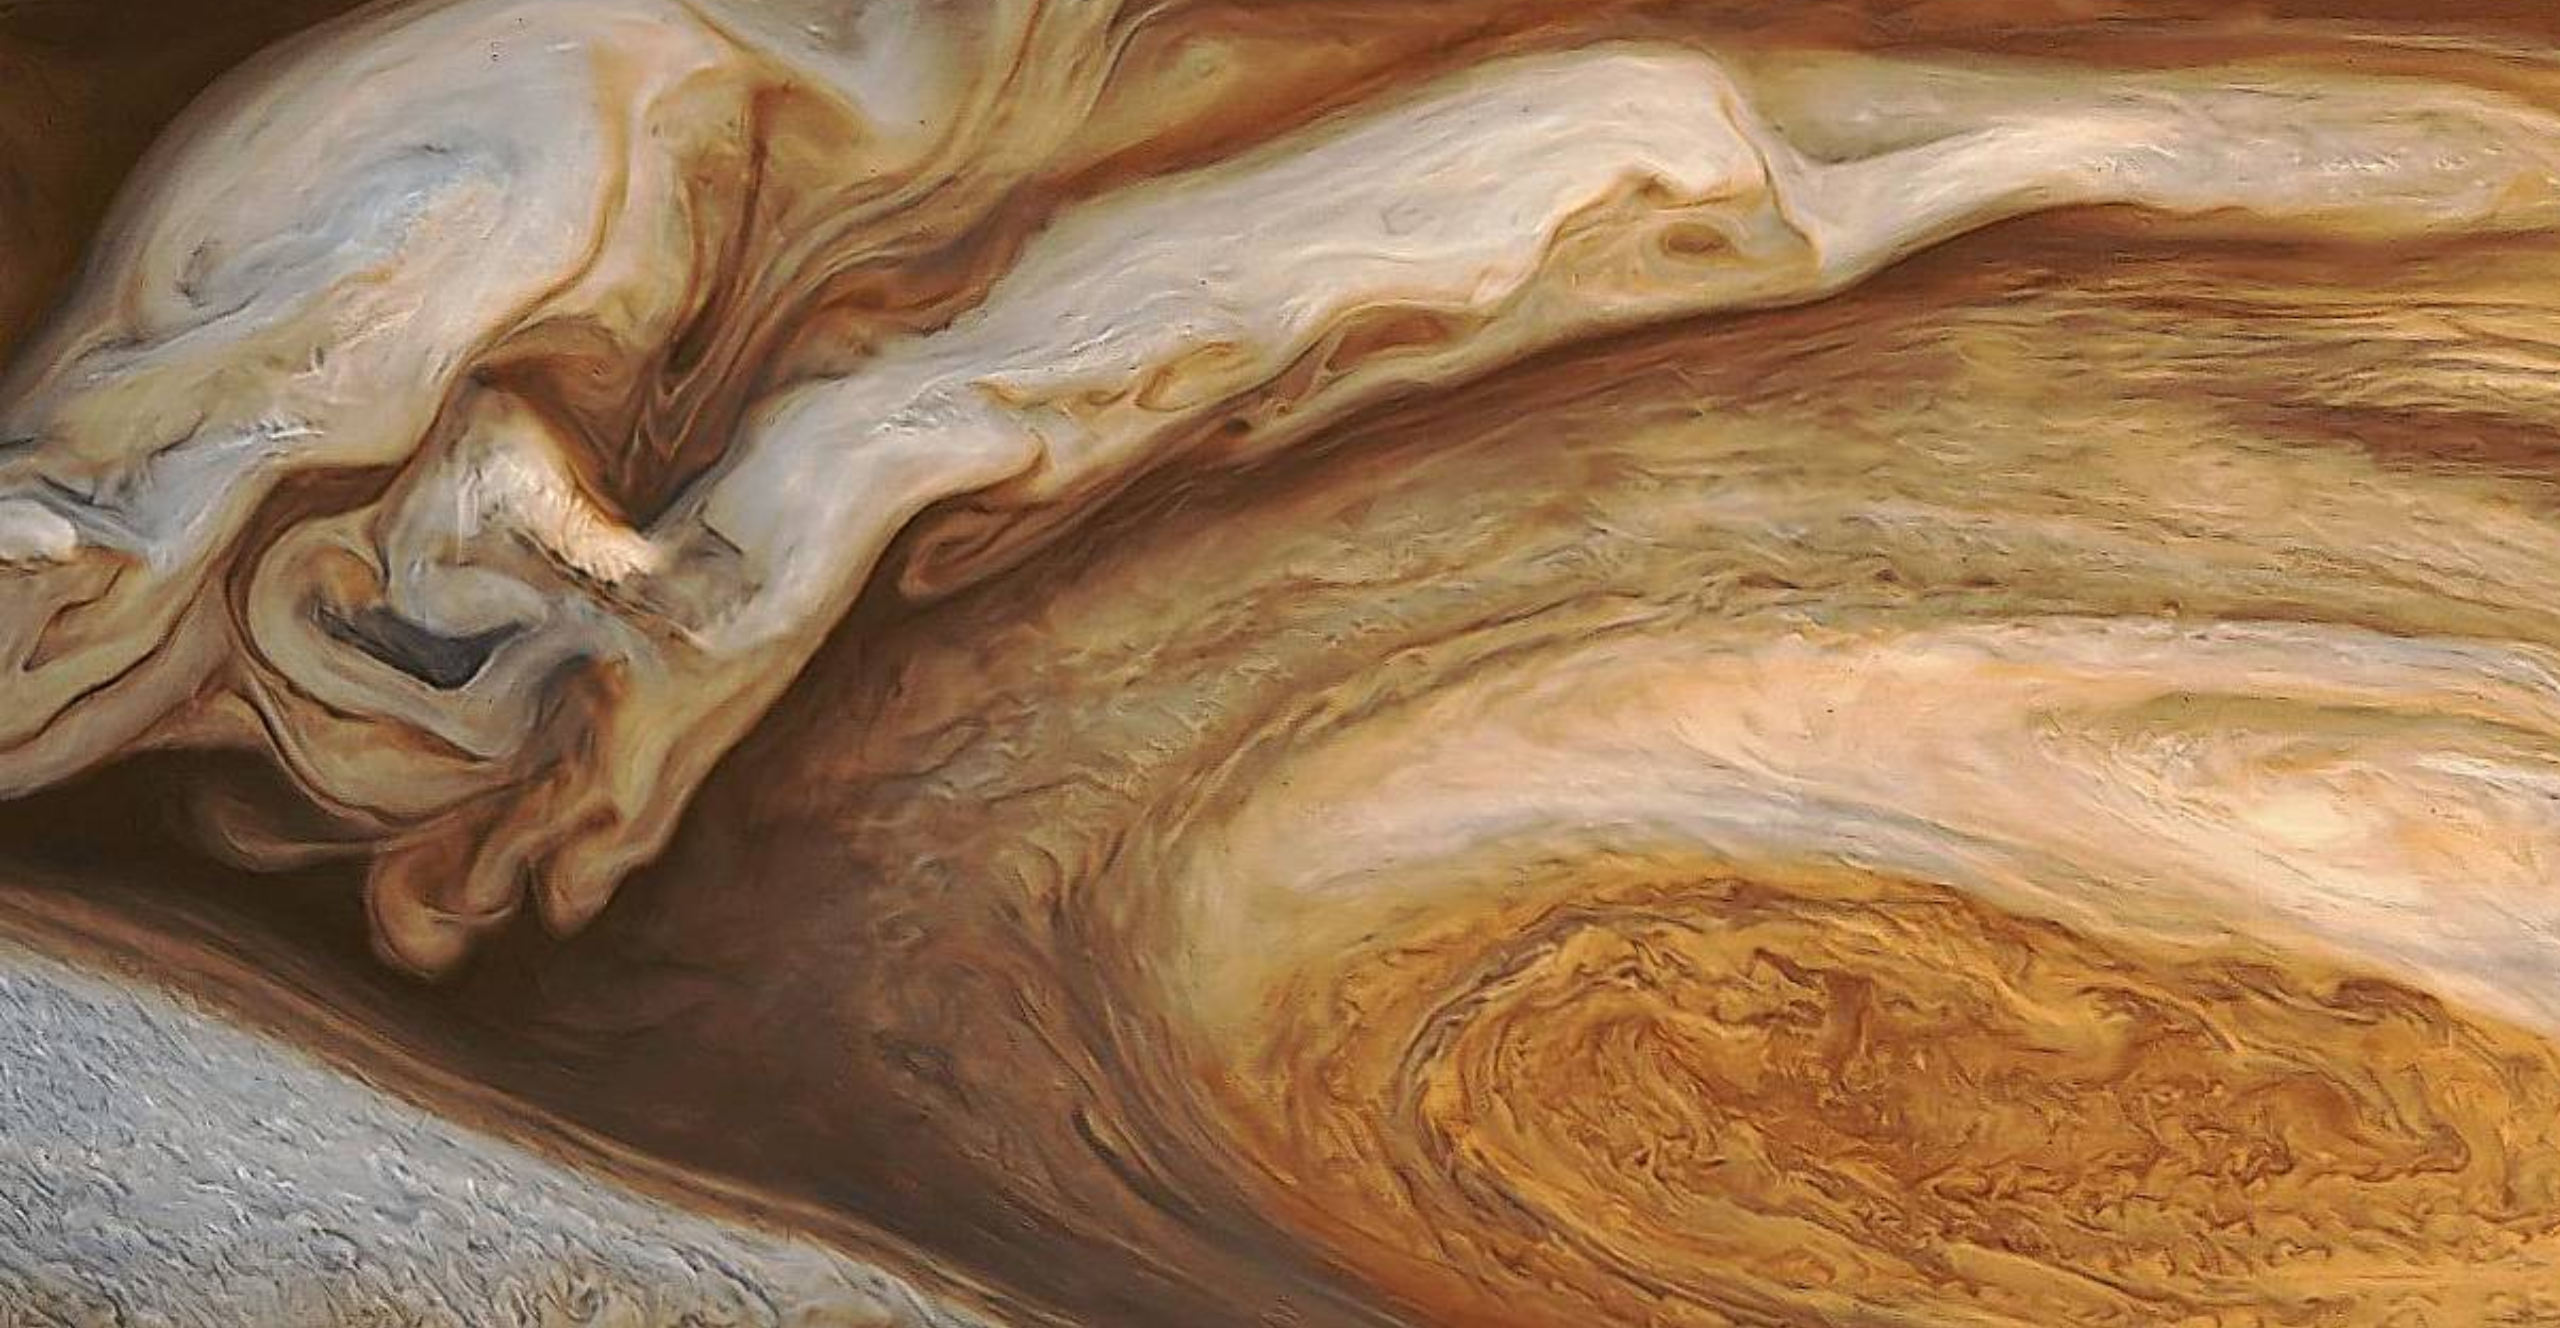
\includegraphics[scale=0.061]{jupiter.png}
				\end{array}
			\end{equation*}
		\end{frame}
		
		\begin{frame}\frametitle{Traditional Hydrodynamics}
			All dynamic and thermodynamic properties of liquids/gas are described by ({\scriptsize Landau\&Lifshitz (1959)})
			\begin{align*}
				\dfrac{\partial \rho}{\partial t}+\nabla(\rho\bm{v})&=0\\
				\rho\left[\dfrac{\partial \bm{v}}{\partial t}+(\bm{v}\cdot\nabla)\bm{v}\right]&=-\nabla p+\eta\nabla^2\bm{v}+\left(\zeta+\dfrac{\eta}{3}\right)\nabla(\nabla\cdot\bm{v})\\
				\rho \left(\dfrac{\partial s}{\partial t}+\bm{v}\cdot\nabla s\right)&=\nabla(\kappa\nabla T)+\dfrac{\eta}{2}\left(\dfrac{\partial v_i}{\partial x_j}+\dfrac{\partial v_j}{\partial x_i}-\dfrac{2}{3}\delta_{ij}\dfrac{\partial v_\ell}{\partial x_\ell}\right)^2+\zeta(\nabla\bm{v})^2.
			\end{align*}
			\only<2>{What hydrodynamic theory does here is to reduce the $6^N$ microscopic degree of freedom $\{\bm{x}_1,\bm{p}_1;\bm{x}_2,\bm{p}_2;\cdots\}$ to just five phenomelogical variable --- velocity field $\bm{v}(\bm{r})$, in-equilibrium density $\rho$ and entropy $s$.}
			\only<3->{
			\vspace{-1em}
			\begin{redblock}{Question}
				\begin{itemize}
					\item Are transport measurements performed in the hydrodynamic regime?
					\item What is the correct low-energy effect degree of freedom?
					\item What is the EOM of such hydro-variables?
					\item How to compute transport coefficients and compare with experiments?
				\end{itemize}
			\end{redblock}}
		\end{frame}
		
\section{Hydrodynamics}
	\subsection{Fundamentals}
		\begin{frame}\frametitle{Assumption of Hydrodynamics}
			\begin{block}{What is Hydrodynamics?}
				``Hydrodynamics is the effective theory describing the relaxation of an interacting classical or quantum system towards thermal equilibrium.''\par\hfill --- {\scriptsize Hartnoll, Lucas, and Sachdev (2018)}
			\end{block}
			We call the relevant fields of such effective field theory \textbf{hydro-variables}.\pause
			\begin{greenblock}{Assumption}
				\begin{itemize}
					\item Hydro-variables consist of conserved quantities and symmetry-breaking fields;
					\item The system reaches thermodynamic equilibrium at each instant of time;
					\item Physical observables are completely determined by hydro-variables.
				\end{itemize}
			\end{greenblock}
			\pause
			To validate the second assumption, we demand the driving frequency of external fields to satisfy ${\color{red}\omega\tau_{\text{th}}\ll1}$, where the natural thermalization time scale ({\scriptsize Damle\&Sachdev, PRB, \textbf{56}, 8714 (1997)}) $\tau_{\text{th}}\sim\hbar/k_B T$. {\color{red}This is the criterion of ``hydrodynamic regime''.}
			
		\end{frame}
		
		\begin{frame}\frametitle{Realization of Hydrodynamic Regime}
			All conductivities are measured at (low) frequency $\omega$ under a low, but \textbf{non-zero temperature} $T$. So we can easily tuned $\omega$ to meet the criterion $\hbar\omega\ll k_B T$.
			\begin{equation*}
				\parbox{4cm}{\centering Transport Coefficients from Hydrodynamics} \Longleftrightarrow \parbox{4cm}{\centering Transport Coefficients from Experiments}.
			\end{equation*}
			\pause
			As a contrast, in finding the universal conductivity around superfluid-insulator transition, for example,
			\begin{itemize}
				\item Many theorerical works ({\scriptsize Fisher \textit{et al.}, PRL, \textbf{64}, 587 (1990); Cha \textit{et al.}, PRB, \textbf{44}, 6883 (1991)}), as well as exact diagnolization ({\scriptsize Runge, PRB, \textbf{45}, 13136 (1992)}), are done at $T=0$ so violate the criterion; 
				\item Even the finite-temperature Numerical Monte Carlo ({\scriptsize Sorensen \textit{et al.}, PRL, \textbf{69}, 828 (1992)}), involving analytic continuation that is insentitive to the temperature range, is questioned to fall out of the correct hydrodynamic regime. 
			\end{itemize}
			\only<3->{
			\begin{redblock}{Advantages of Hydrodynamic Theory}
				It provides simple, direct, and novel predictions/explanations to experiments that microscopic calculation hard to cover.
			\end{redblock}}
		\end{frame}
		
	\subsection{Magnetotransport in LSCO: Relativistic Hydrodynamics}
		\begin{frame}\frametitle{Nernst Signal of $\mathrm{La}_{2-x}\mathrm{Sr}_x\mathrm{CuO}_4$}
			\begin{columns}
				\begin{column}{0.3\textwidth}
					\begin{figure}[!htp]
						\centering
						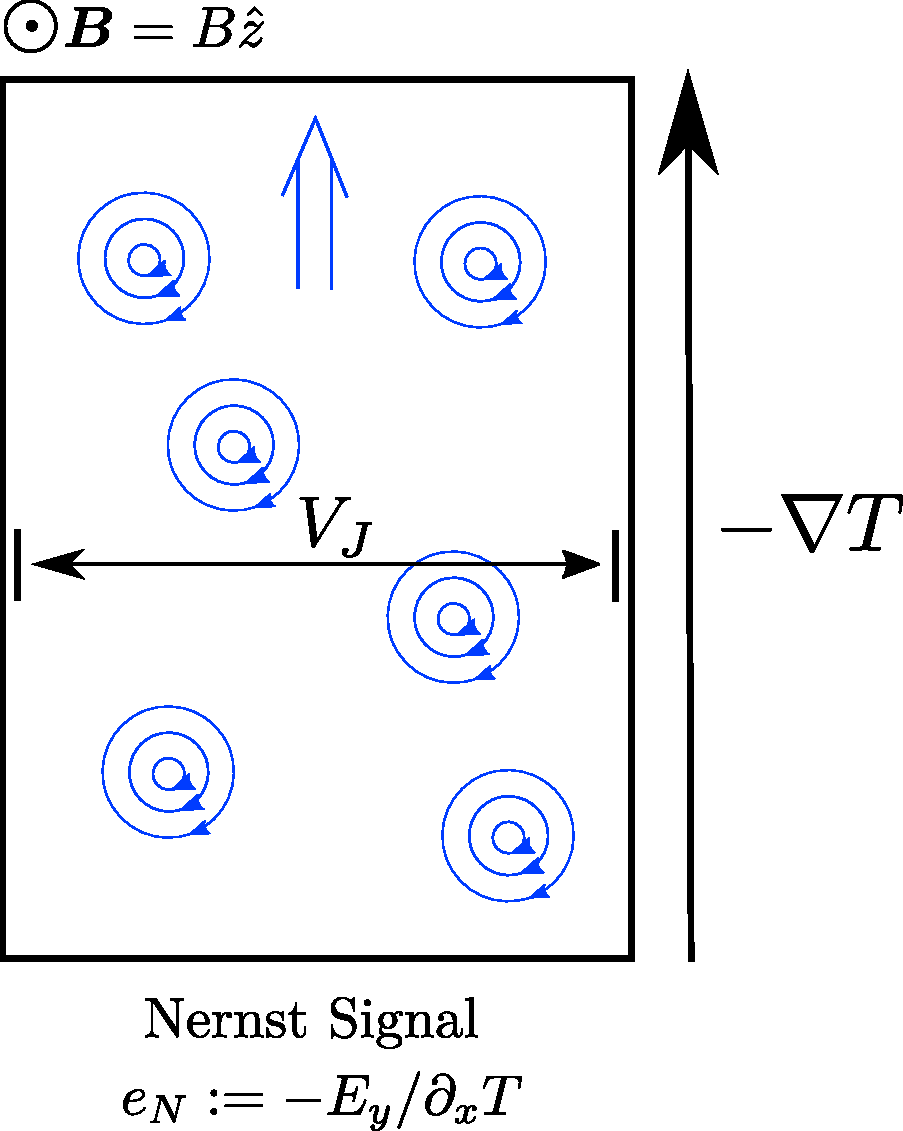
\includegraphics[scale=0.25]{vortex.pdf}
						%\caption{Extrated from {\scriptsize Barišić \textit{et al.} PNAS, \textbf{110}, 30 (2013)}.}
					\end{figure}
				\end{column}
				\begin{column}{0.7\textwidth}
					\begin{figure}[!htp]
						\centering
						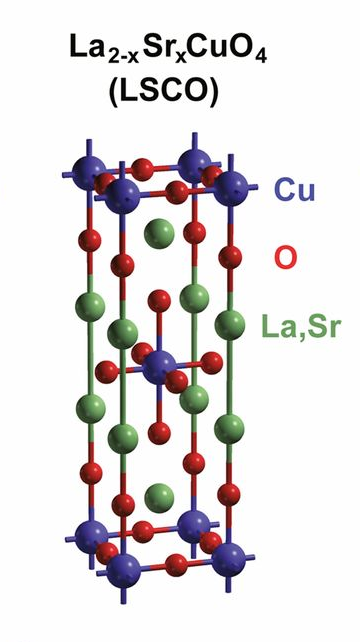
\includegraphics[scale=1]{SC.png}
						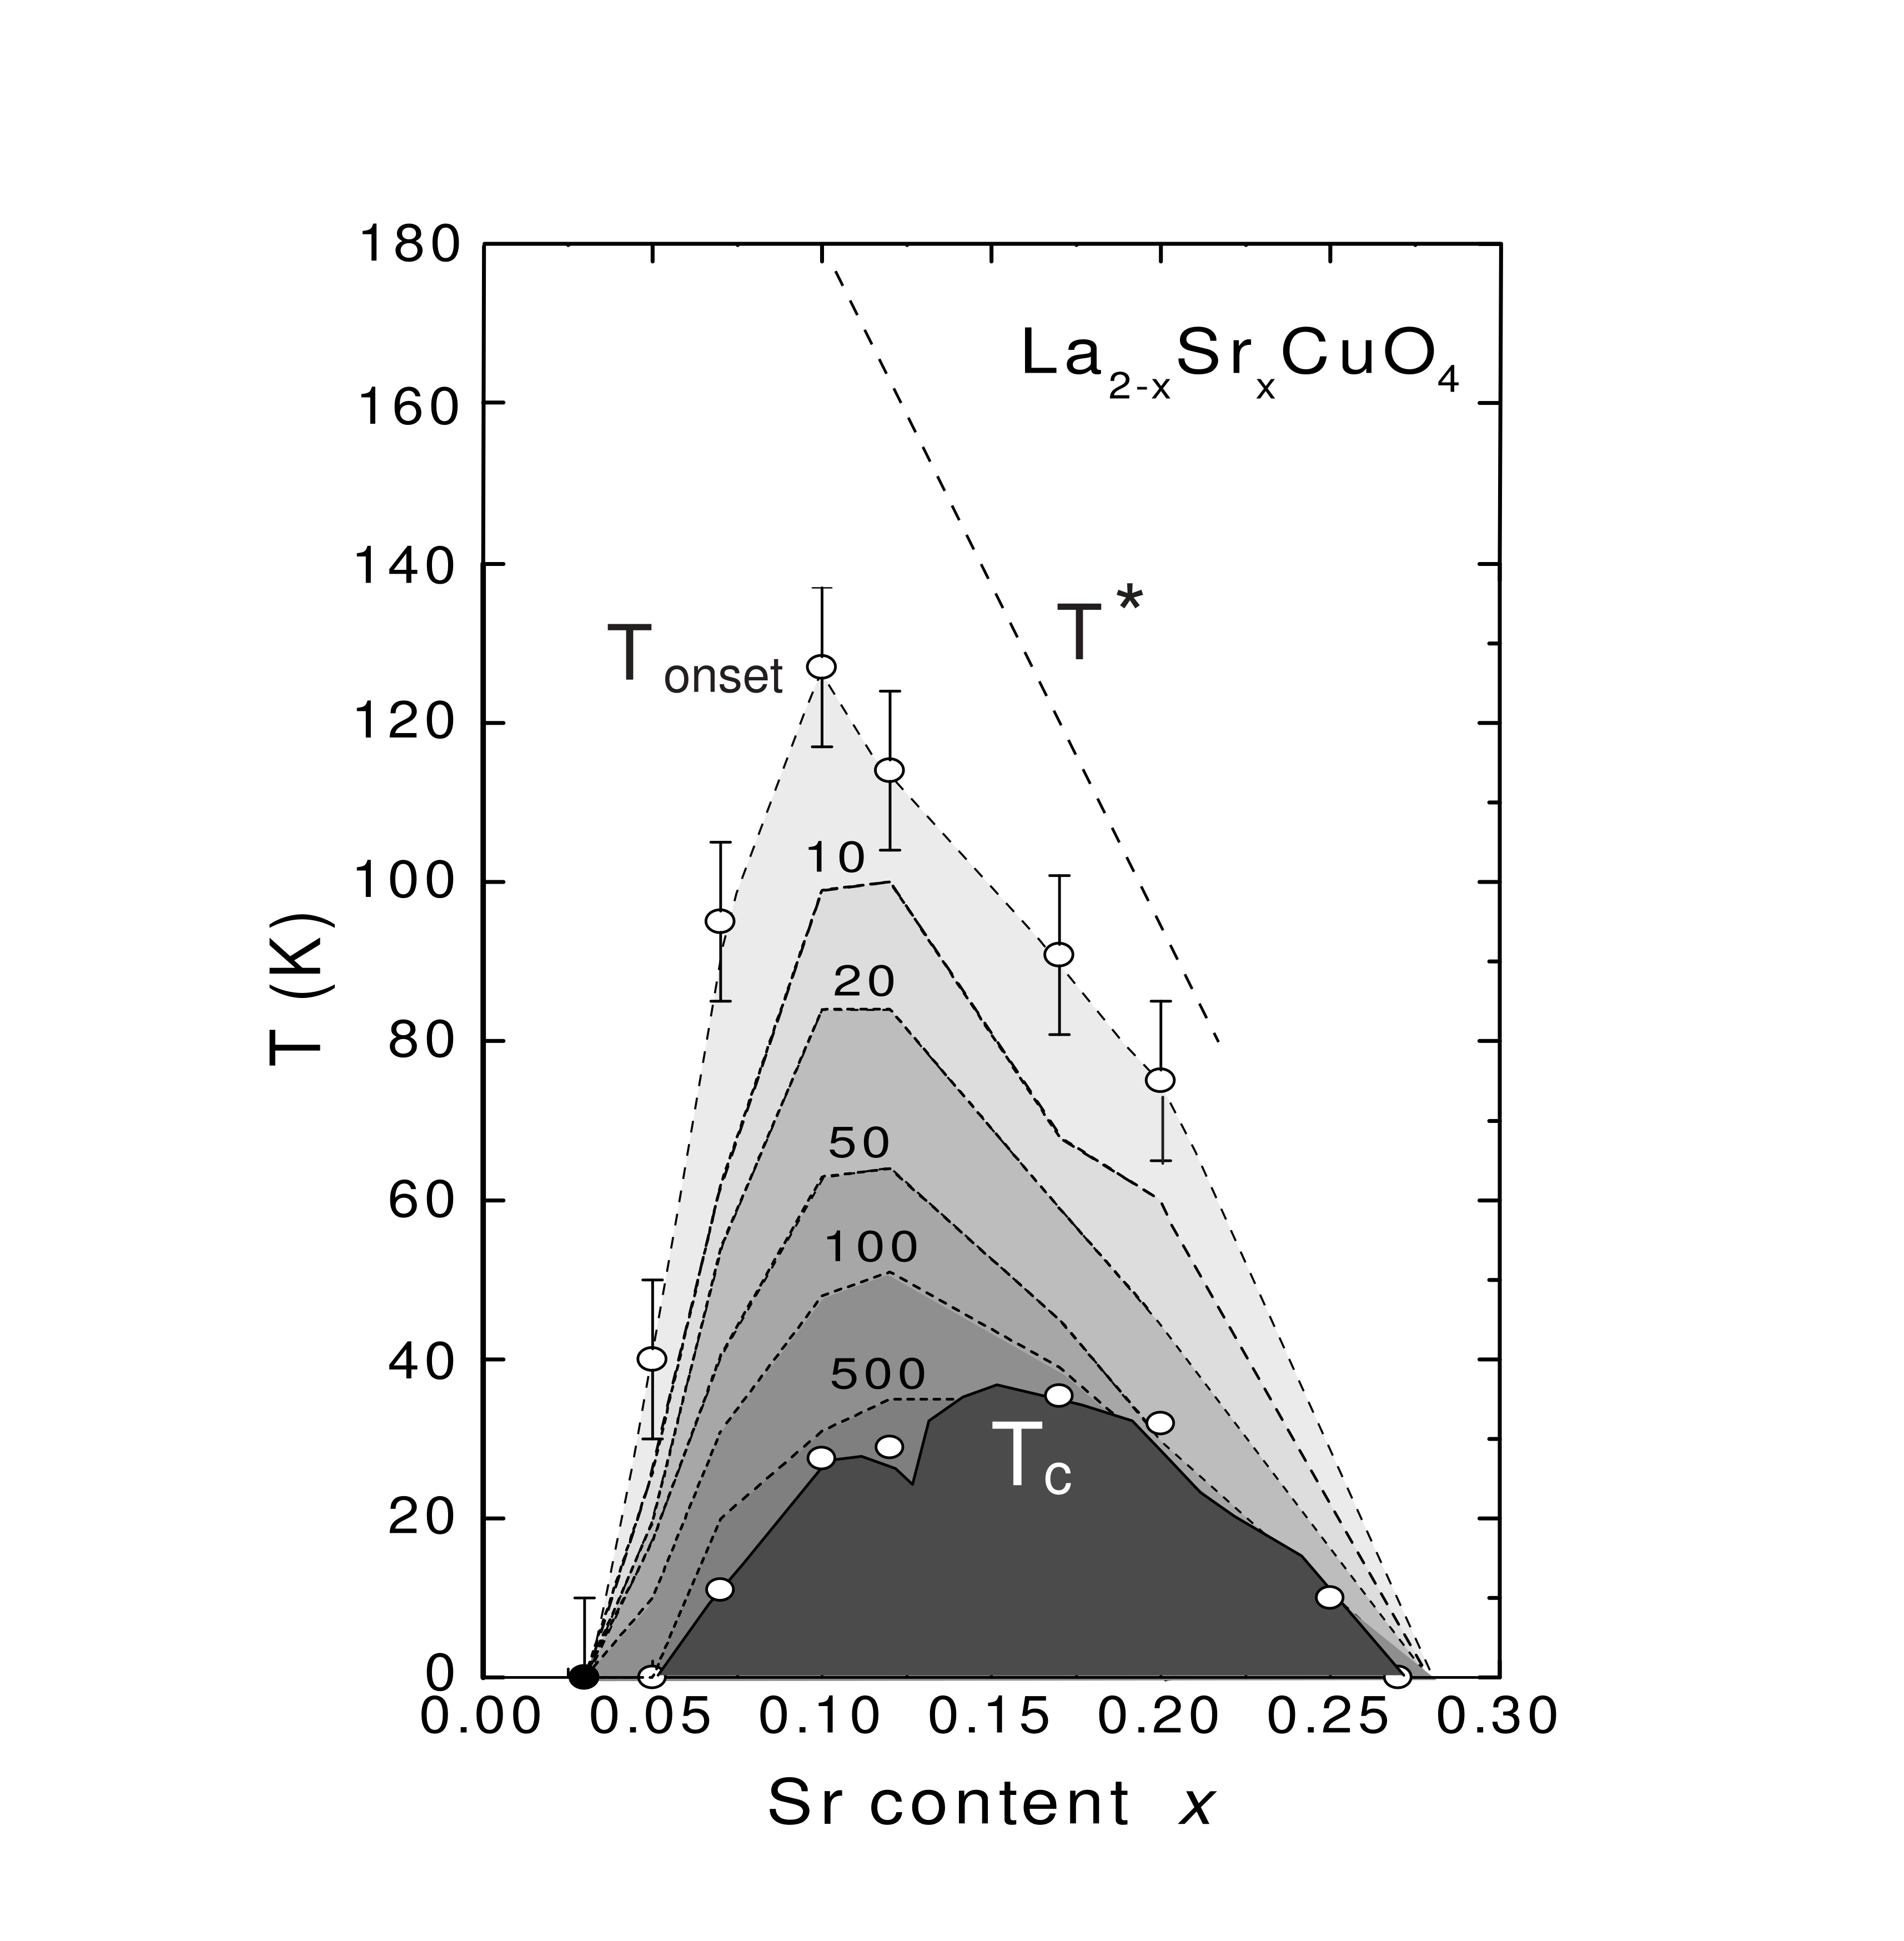
\includegraphics[scale=0.6]{LSCO.png}
						\caption{\textbf{Lattice Structure and Phase diagram of LSCO}. The Nernst coefficient on Contour $\nu\equiv e_N/B$. Extracted from {\scriptsize Wang \textit{et al.} PRB, \textbf{73}, 024510 (2006)}.}
					\end{figure}
				\end{column}
			\end{columns}
		\end{frame}
		\begin{frame}\frametitle{Quantum Criticality}
			\begin{columns}
				\begin{column}{0.5\textwidth}
					\only<1>{\begin{figure}[!htp]
						\centering
						\includegraphics[scale=0.5]{kumagai1994.png}
						\caption{Sharp drop of the superconducting transition temperature. Extracted from {\scriptsize Kumagai \textit{et al.}, J. Superconductivity, \textbf{7}, 1 (1993)}}
					\end{figure}}
					\only<2>{
						\begin{itemize}
							\item Zero field $\mu$SR measurements provide evidence for AFM order of Cu moments ({\scriptsize Kumagai \textit{et al.}, J. Superconductivity, \textbf{7}, 1 (1993)})
							\item Elastic/Inelastic Neutron Scattering reveals magnetically ordered SDW states ({\scriptsize Yamada \textit{et al.}, PRB, \textbf{57}, 6165 (1998)})
							\item 14keV (Hard) X-ray diffraction measurements reveals CDW states ({\scriptsize Croft \textit{et al.}, PRB, \textbf{89}, 224513 (2014)})
						\end{itemize}
					}
					\only<3->{
						\vspace{-1.5em}
						\begin{figure}[!htp]
							\centering
							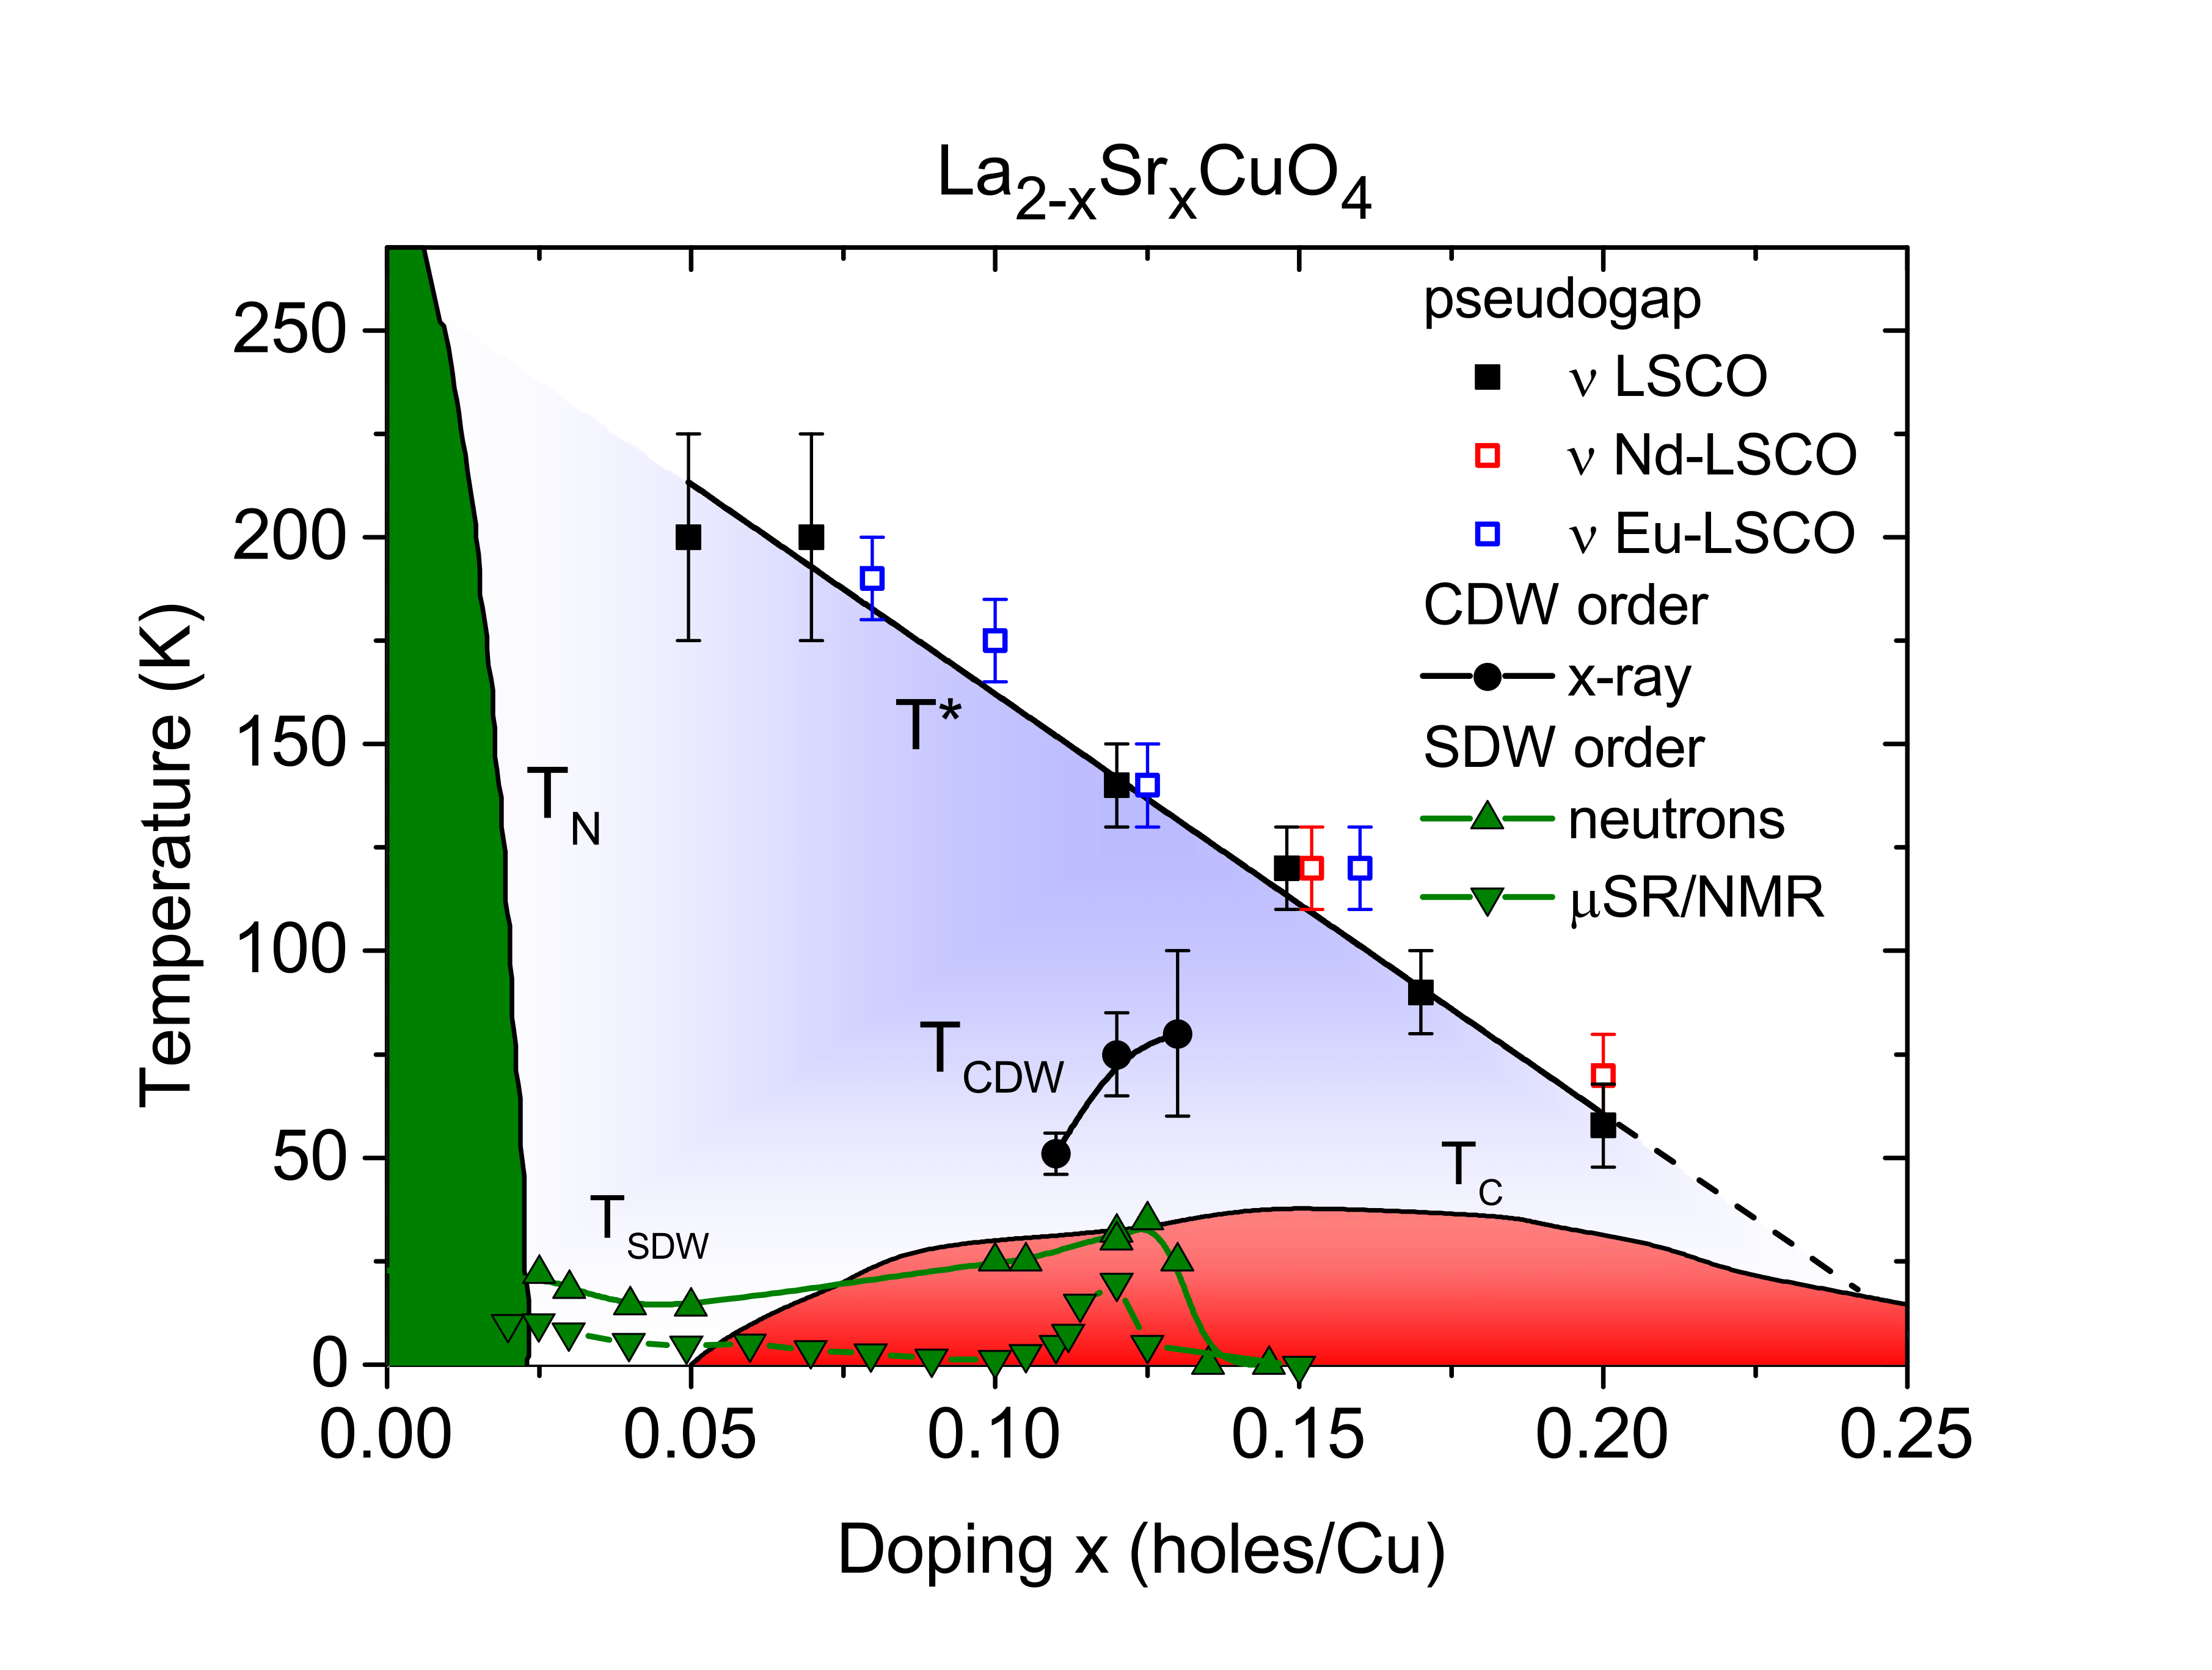
\includegraphics[scale=0.7]{CDW.png}
							\caption{Onset temperature of each type of experiment in LSCO phase diagram. Extracted from {\scriptsize Croft \textit{et al.}, PRB, \textbf{89}, 224513 (2014)}.}
						\end{figure}
						
					}
				\end{column}
				\begin{column}{0.4\textwidth}
					\begin{figure}[!htp]
						\centering
						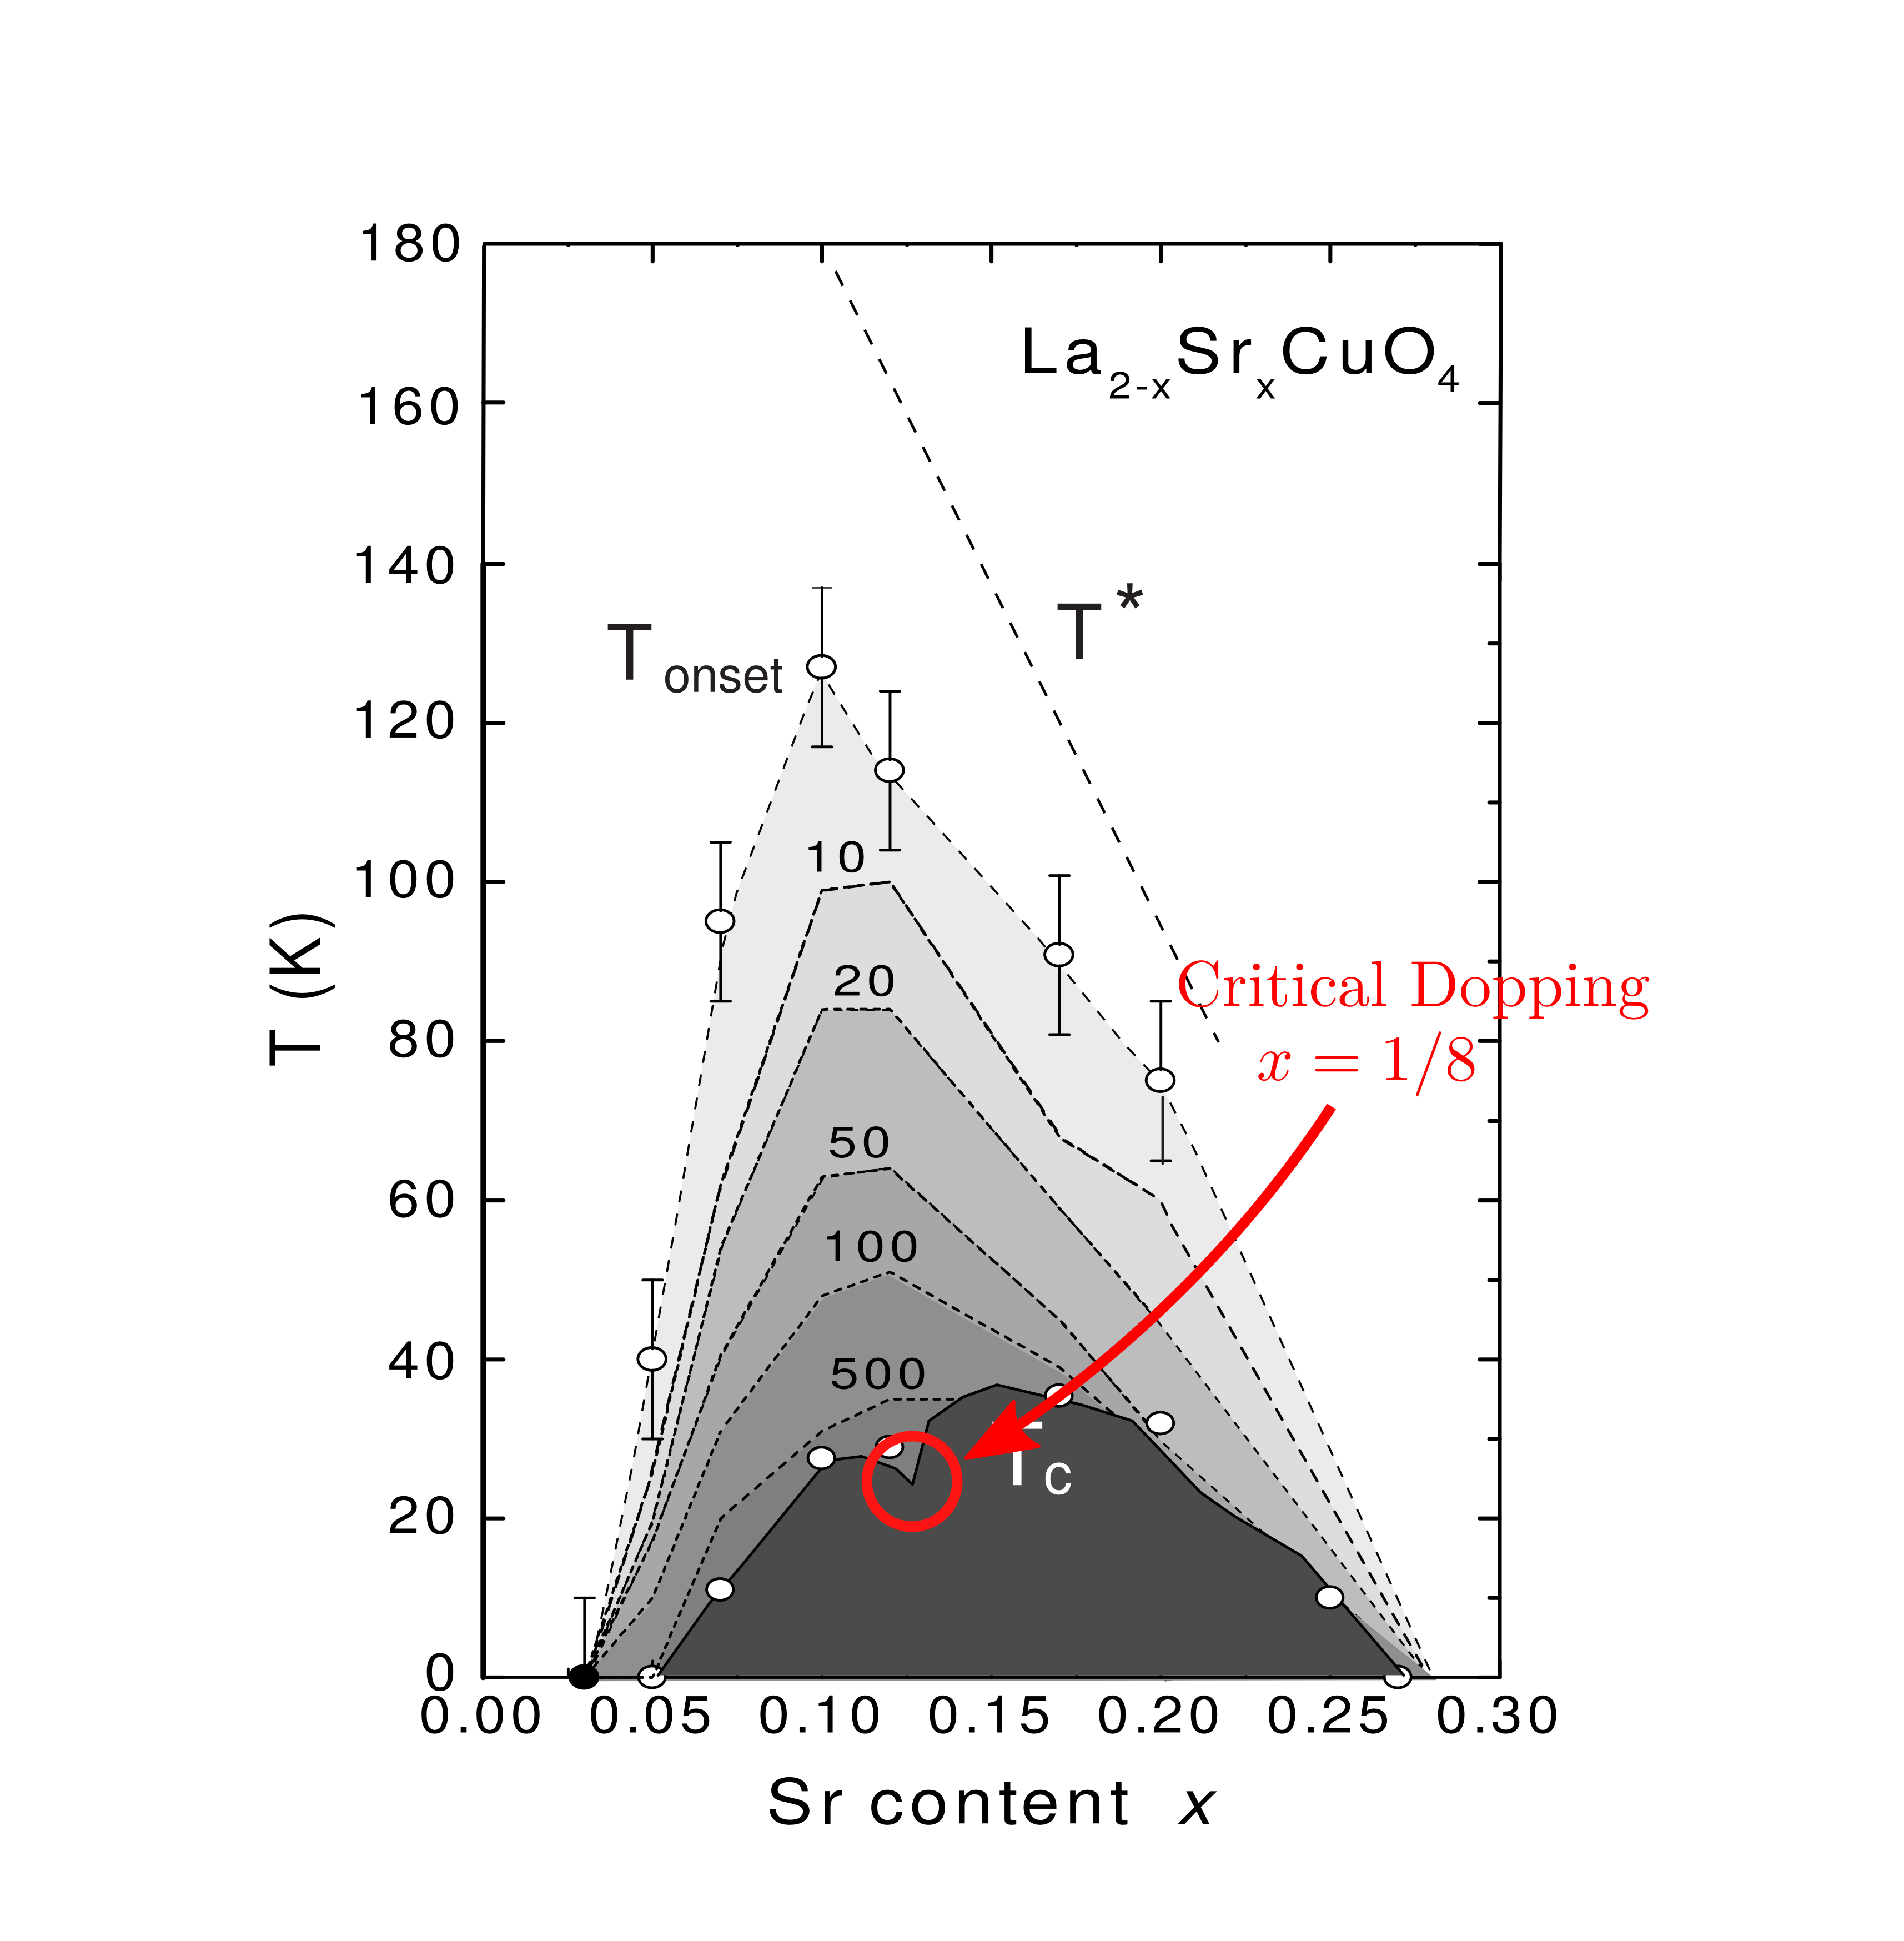
\includegraphics[scale=0.04]{LSCO-2.png}
					\end{figure}
					\only<4>{\vspace{-1em}\color{red} Physics close to the sharp dip around doping $x=1/8$ demands a quantum critical theory, or CFT.}
				\end{column}
			\end{columns}
		\end{frame}		
		
		\begin{frame}\frametitle{Bose-Hubbard Model}
			\begin{columns}
				\begin{column}{0.45\textwidth}
					The simplest model for superfluid-insulator phase transition of vortice liquid is
					\begin{block}{Bose-Hubbard Model}
						\begin{align*}
							H&=-t\sum_{\langle ij \rangle}b_i^\dagger b_j-\mu\sum_i n_i\\
							&\quad+\dfrac{U}{2}\sum_i n_i(n_i-1)
						\end{align*}
					\end{block}
				\end{column}
				\begin{column}{0.5\textwidth}
					\begin{figure}[!htp]
						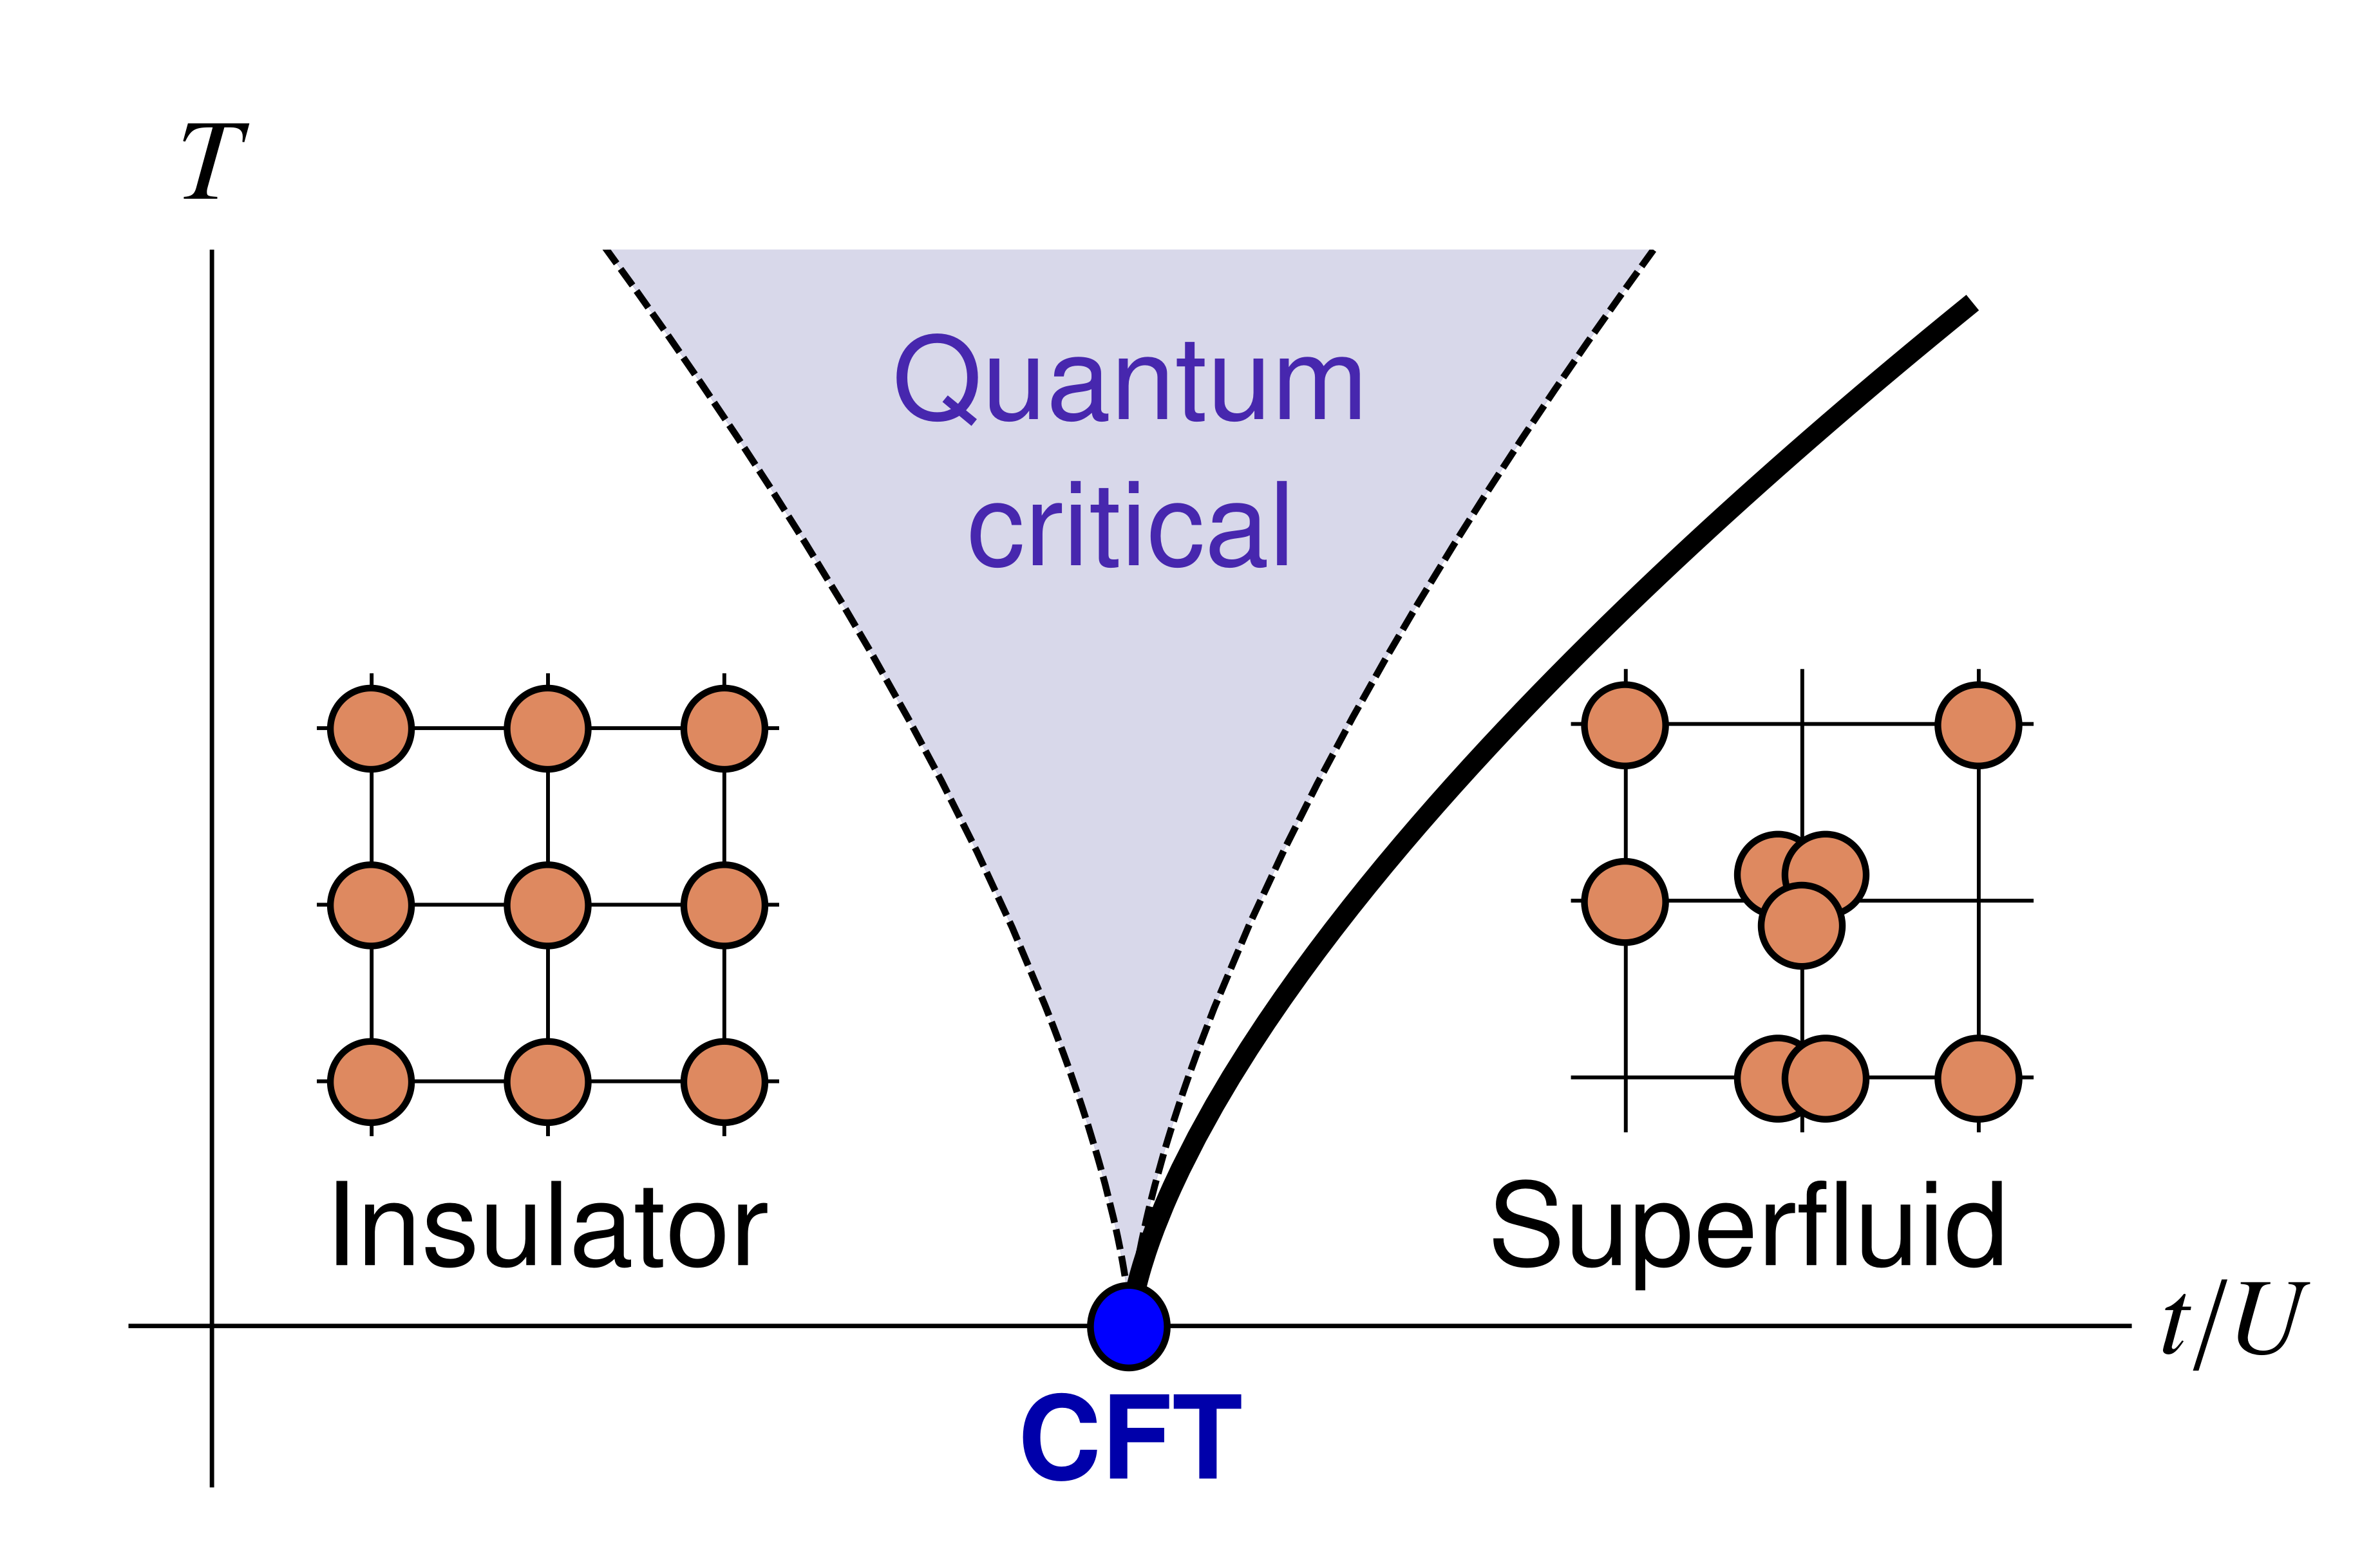
\includegraphics[scale=0.5]{Witczak.png}
						\caption{Extracted from {\scriptsize Witczak-Krempa \textit{et al.}, Nat. Phys., \textbf{10}, 5 (2014)}.}
					\end{figure}
				\end{column}
			\end{columns}
			\pause
			And the critical theory is given by ({\scriptsize Fisher \textit{et al.}, PRB, \textbf{40}, 1 (1989)})
			\begin{redblock}{(2+1)-D Conformal Field Theory}
				\begin{equation*}
					S=\int\dd^2r\dd\tau\bigg[|\partial_\tau\psi|^2+v^2|\nabla\psi|^2-g|\psi|^2+\dfrac{u}{2}|\psi|^4\bigg].
				\end{equation*}
			\end{redblock}
			%In the application of cuprates, the Mott insulator phase shrink to just one point of hole density $x=1/8$.
		\end{frame}

		\begin{frame}\frametitle{Linear Response Around Critical Point}
			\begin{columns}
				\begin{column}{0.5\textwidth}
					To study the Nernt effect of LSCO (dotted line on the RHS), we are going to perturb such CFT with 
					\begin{itemize}
						\item a chemical potential fluctuation $-\nabla\mu$ (induced by external electric fields)
						\item an external magnetic field $B$
						\item a thermal fluctuation $-\nabla T$
						\item a small density of impurities
					\end{itemize}
					and calculate the corresponding linear reponses.
				\end{column}
				\begin{column}{0.4\textwidth}
					\vspace{-1.5em}
					\begin{figure}[!htp]
						\centering
						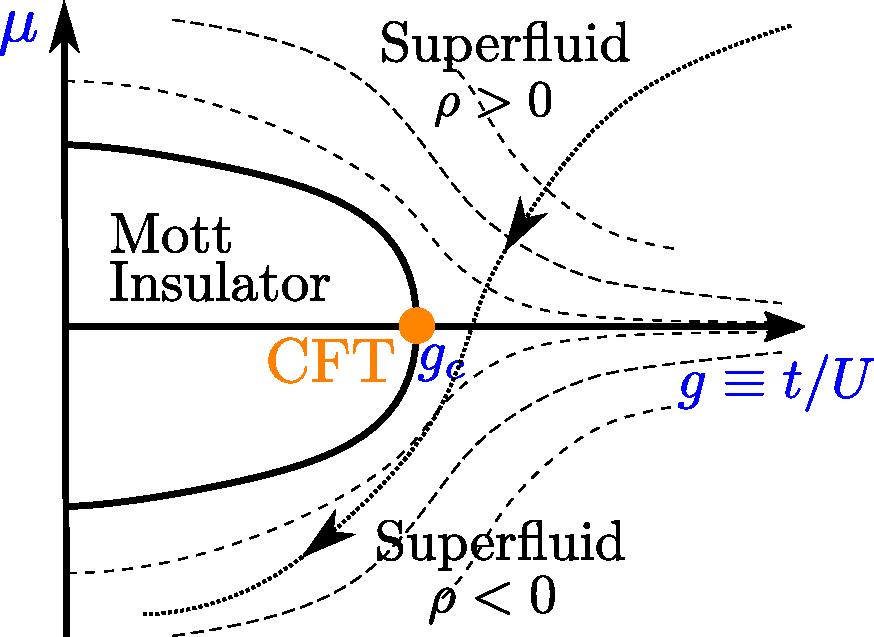
\includegraphics[scale=0.35]{CFT.pdf}
					\end{figure}
					
				\end{column}
			\end{columns}

			\begin{block}{Perturbative CFT}
				\begin{equation*}
					S=\int\dd^2r\dd\tau\bigg[|\partial_\tau-\mu\psi|^2+v^2|(\nabla-i2e\bm{A})\psi|^2-g|\psi|^2+\dfrac{u}{2}|\psi|^4+\mathcal{L}_{\text{imp}}\bigg].
				\end{equation*}
			\end{block}
		\end{frame}

		\begin{frame}\frametitle{Conservation Law}
			The Lorentz-invariant microscopic action gives rise to two \emph{macroscopic} \textbf{Ward identities} ({\scriptsize Herzog, J. Phys. A, \textbf{42}, 34 (2009)}) (as \textbf{\color{red}conservation laws})
			\begin{redblock}{Conservation Laws}
				\begin{equation*}
					\nabla_\mu\langle T^{\mu\nu}\rangle=F^{\nu\lambda}\langle J_\lambda\rangle,\quad \partial_\mu\langle J^\mu\rangle=0,
				\end{equation*}
			\end{redblock}
			where
			\begin{itemize}
				\item (macroscopic) current operator $\langle J^\mu\rangle\equiv-\dfrac{\delta}{\delta A_\mu}W[g,A]$,
				\item (macroscopic) stress-energy tensor $\langle T^{\mu\nu}\rangle\equiv=\dfrac{-2}{\sqrt{g}}\dfrac{\delta}{\delta g_{\mu\nu}}W[g,A]$,
				\item $W[g,A]$ is the generating functional
			\end{itemize}
			\only<2->{
				\begin{redblock}{Hydro-variables}
					By assumption, we thus have three (dual) hydro-variables: chemical potential $\mu$, temperature $T$, and (normalized) velocity $u^\mu$. 
				\end{redblock}
			}
		\end{frame}

		\begin{frame}\frametitle{Constitutive Relation --- Zeroth Order}
			By {\scriptsize Eckart, Phys. Rev., \textbf{58}, 10 (1940)}, given a vector $u^\mu$, one can always decompose the two tensors with the projection operator $P^{\mu\nu}=g^{\mu\nu}+u^\mu u^\nu$ that
			\begin{align*}
				J^\mu&=\mathcal{N}u^\mu+j^\mu,\\
				T^{\mu\nu}&=\mathcal{E}u^\mu u^\nu+\mathcal{P}P^{\mu\nu}+(q^\mu u^\nu+q^\nu u^\mu)+t^{\mu\nu},
			\end{align*}
			where scalar $\mathcal{N}$, $\mathcal{E}$, and $\mathcal{P}$, vector $j^\mu$ and $q^\nu$, and tensor $t^{\mu\nu}$ are formally contractions with whether velocity vector or projection operator
			\only<1>{
			\begin{align*}
				\parbox{3cm}{\centering scalar}\quad\mathcal{N}&\equiv J^\mu u_\mu,\quad\mathcal{E}\equiv T^{\mu\nu}u_\mu u_\nu,\quad\mathcal{P}\equiv P^{\mu\nu}T_{\mu\nu},\\
				\parbox{3cm}{\centering {\color{red}transverse} vector}\quad j^\mu&\equiv P^{\mu\nu}J_\nu,\quad q^\mu\equiv-P^{\mu\nu}u^\rho T_{\nu\rho},\\
				\parbox{3cm}{\centering {\color{red}transverse-traceless} tensor}\quad t_{\mu\nu}&\equiv\dfrac{1}{2}\left(P_{\mu \alpha}P_{\nu\beta}+P_{\alpha\nu}P_{\mu\beta}-\dfrac{2}{d}P_{\mu\nu}P_{\alpha \beta}\right)T^{\alpha \beta} 
			\end{align*}
			}
			
			\only<2->{
			Choosing the proper frame of reference, we get the familiar constitutive relation of ideal fluids
			\begin{block}{Zeroth Order}
				\begin{equation*}
					\mathcal{N}=\rho(T,\mu),\quad \mathcal{E}=\varepsilon(T,\mu)+P(T,\mu),\quad\mathcal{P}=P(T,\mu).
				\end{equation*}
			\end{block}
			so that accidentally \textbf{\color{red}the entropy current is conserved}
			\begin{equation*}
				{\color{red}\partial_\mu s^\mu\equiv \partial_\mu (su^\mu)=0.}
			\end{equation*}
			}
		\end{frame}
		
		\begin{frame}\frametitle{Constitutive Relation --- First Order}
			\begin{redblock}{Subtleties on ``Frame Choice'' ({\scriptsize Kovtun, J. Phys. A, \textbf{45}, 47 (2012)})}
				The notion of local hydro-variables $\{T,\mu,u^\mu\}$ are NOT uniquely defined up to the conservation laws.
			\end{redblock}
			Generally,
			\begin{equation*}
				\begin{cases}
					T(\bm{r})\mapsto T'(\bm{r})\equiv T+\delta T,\\
					\mu(\bm{r})\mapsto \mu'(\bm{r})\equiv \mu+\delta \mu,\\
					u^\mu(\bm{r})\mapsto {u^\mu}'(\bm{r})\equiv u^\mu+\delta u^\mu,
				\end{cases}\Longrightarrow
				\begin{cases}
					\delta\mathcal{E}=\delta\mathcal{P}=\delta\mathcal{N}=0,\\
					\delta j^\mu\simeq -\mathcal{N}\delta u^\mu,\quad\delta q^\mu\simeq (\varepsilon+P)\delta u^\mu,\\
					\delta t^{\mu\nu}\simeq 0.
				\end{cases}
			\end{equation*}
			Even the zeroth-order constitutive relation will suffer from such redefinition!
			\only<2->{
			\begin{block}{Gauge fix of the first-order spatial gradient expansion}
				\begin{itemize}
					\item We choose $\delta T$ and $\delta\mu$ such that $\mathcal{E}\equiv \varepsilon$ and $\mathcal{N}\equiv\rho$;
					\item We choose $\delta u^\mu$ such that the first-order $q^\mu\equiv 0$ (\textbf{Landau Frame}).
				\end{itemize}
			\end{block}
			}
		\end{frame}
		
		\begin{frame}\frametitle{Constitutive Relation --- First Order}
			List all possible terms allowed by symmetry as following ({\scriptsize Bhattacharya \textit{et al.}, JHEP, \textbf{05}, 147 (2014)})\\
			(here we assume \textbf{time-reversal symmetry} and \textbf{parity-inversion symmetry})
			\begin{center}
				\begin{tabular}{c||c|c|c}
					& All Data & EOM & {\color{red}Independent Data}\\
					\hline\hline
					Scalars & $u^\mu \partial_\mu T, u_\mu \partial_\mu \mu, \partial_\mu u^\mu$ & $u_\mu\nabla_\nu T^{\mu\nu}=0$ & {\color{red}$\partial_\mu u^\mu$ }\\
					& & $\partial_\mu J^\mu=0$ & \\
					\hline
					Transerves & $P^{\mu\nu} \partial_\nu T, P^{\mu\nu}\partial_\nu\mu$ & $P^{\mu\nu}\nabla^\lambda T_{\mu\nu}=0$ & {\color{red}$P^{\mu\nu}\partial_\nu T, P^{\mu\nu}\partial_{\nu\mu}$}\\
					Vectors & $P^{\mu\nu}u^\lambda \partial_\lambda u_\nu, F^{\mu\nu}u_\nu$ & & {\color{red}$F^{\mu\nu}u_\nu$} \\
					\hline
					Transverse- & $\sigma^{\mu\nu}\equiv P^{\mu \alpha}P^{\nu\beta}$ & & \\
					traceless & $\bigg(\partial_\alpha u_\beta+\partial_\beta u_\alpha$ & &  {\color{red}$\sigma^{\mu\nu}$} \\
					Tensor & $-\dfrac{2}{d}g_{\alpha\beta}\partial_\lambda u^\lambda\bigg)$ & &
				\end{tabular}
			\end{center}
		\end{frame}

		\begin{frame}\frametitle{Constitutive Relation --- First Order}
			Combine all possible terms linearly, we get
			\begin{block}{First Order}
				\vspace{-1em}
				\begin{align*}
					j^\mu&=-\sigma_Q TP^{\mu\nu}\partial_\nu\left(\dfrac{\mu}{T}\right)-\chi_T P^{\mu\nu}\partial_\nu T,&\sigma_Q:\text{Universal Conductivity}\\
					\mathcal{P}&=P-\zeta \partial_\lambda u^\lambda,&\zeta:\text{Bulk Viscosity}\\
					t^{\mu\nu}&=-\eta P^{\mu\alpha}P^{\nu\beta}\bigg(\partial_\alpha u_\beta+\partial_\beta u_\alpha-\dfrac{2}{2}g_{\alpha\beta}\partial_\lambda u^\lambda\bigg).&\eta:\text{Shear Viscosity}
				\end{align*}
			\end{block}
			\pause
			The constraint of {\color{red}non-negative entropy production}
			\begin{equation*}
				\partial_\mu S^\mu\equiv \partial_\mu \left(su^\mu+\dfrac{\mu}{T}J^{(1)\mu}\right) =-J^{(1)\mu}\partial_\mu \left(\dfrac{\mu}{T}\right)-\dfrac{1}{T}T^{(1)\mu\nu}\partial_\nu u_\mu\geq0
			\end{equation*}
			requires
			\begin{equation*}
				\chi_T\equiv0,\quad \zeta>0,\quad \sigma_Q>0,\quad\eta>0. 
			\end{equation*}

		\end{frame}
		
		\begin{frame}\frametitle{Hydrodynamic EOM}
			Following {\scriptsize Kandanoff\&Martin, Ann. Phys., \textbf{24}, 419 (1969)}, the linear response over equilibrium state can be obtained by introducing a purtabative Hamiltonian
			\begin{equation*}
				\mathcal{H}\rightarrow\mathcal{H}-\int\dd^{2}x\,\left(\dfrac{\delta T}{T}(\varepsilon-\mu\rho)+\delta \mu\rho+\delta u^\mu T_{\mu0}\right),
			\end{equation*}
			where we explicitly split out the perturbative source of energy density, charge density, and momentum densities.\\
			\pause
			Linearized Hydrodynamic equations of motion are read out from conservation laws
			\begin{block}{Conservation Laws}
				\vspace{-1em}
				\begin{align*}
					\partial_t\rho+\nabla\cdot\bigg\{\rho\bm{v}+\sigma_Q\left[-\nabla\mu+\dfrac{\mu}{T}\nabla T+\bm{v}\times\bm{B}\right]\bigg\}&=0\\
					\partial_t\varepsilon+\nabla\cdot\bigg((\varepsilon+P)\bm{v}\bigg)&=0\\
					\partial_t\bigg((\varepsilon+P)\bm{v}\bigg)+\nabla p-\zeta\nabla(\nabla\cdot\bm{v})-\eta\nabla^2\bm{v}-\delta\bm{J}\times B&=0.
				\end{align*}
			\end{block}
		\end{frame}

		\begin{frame}\frametitle{Thermoelectric Response}
			Thermoelectric response coefficients are defined as		
			\begin{equation*}
				\left(\begin{array}{c}
					\bm{J}\\\bm{Q}
				\end{array}\right)=\left(\begin{array}{cc}
					\bm{\sigma}&\bm{\alpha}\\T\bm{\alpha}&\bm{\bar{\kappa}}
				\end{array}\right) \left(\begin{array}{c}
					-\nabla\mu\\-\nabla T
				\end{array}\right), 
			\end{equation*}
			where electric field $\bm{E}=-\nabla\mu$. We are also interested in 
			\begin{itemize}
				\item \textbf{Thermal Conductivity}: heat current induced by thermal gradient but in the absence of charge current $\bm{Q}=-\bm{\kappa}\nabla T$. So $\bm{\kappa}\equiv\bm{\bar{\kappa}}-T\bm{\alpha}\bm{\sigma}^{-1}\bm{\alpha}$,
				\item \textbf{Nernst Response}: electric field induced by thermal gradient but in the absense of charge current $\bm{E}=-\bm{\theta}\nabla T$. So $\bm{\theta}\equiv-\bm{\sigma}^{-1}\bm{\alpha}$.
			\end{itemize}
			\pause
			All of them can be obtained after a lengthy re-arrangement of hydrodynamic EOM, with the poles
			\begin{block}{\textbf{Cyclotron Resonance}}
				\begin{equation*}
					\omega=\pm\omega_c+i\gamma,\quad \omega_c\equiv\dfrac{v^2}{c^2}\dfrac{2B}{(\varepsilon+P)/\rho c},\quad \gamma\equiv\sigma_Q\dfrac{v^2}{c^2}\dfrac{B^2}{\varepsilon+P}.
				\end{equation*}
			\end{block}
		\end{frame}

		\begin{frame}\frametitle{Thermoelectric Response}
			On the aspect of ``particle'',
				\begin{align*}
					\sigma_{xx}&=\sigma_Q\dfrac{\omega+i\gamma+i\omega_c^2/\gamma}{(\omega+i\gamma)^2-\omega_c^2},&\sigma_{xy}&=-\dfrac{\rho}{B}\dfrac{\gamma^2+\omega_c^2-2i\gamma\omega}{(\omega+i\gamma)^2-\omega_c^2},\\
					\alpha_{xx}&=\dfrac{\rho}{T}\dfrac{i\omega}{(\omega+i\gamma)^2-\omega_c^2},&\alpha_{xy}&=-\dfrac{\gamma}{B}\dfrac{\gamma^2+\omega_c^2-i\gamma\omega}{(\omega+i\gamma)^2-\omega_c},\\
					\bar{\kappa}_{xx}&=s\dfrac{i\omega-\gamma}{(\omega+i\gamma)^2-\omega_c^2},&\bar{\kappa}_{xy}&=-s\dfrac{\omega_c}{(\omega+i\gamma)-\omega_c^2},
				\end{align*}
			while on the aspect of ``vortex'',
			\begin{align*}
				\rho_{xx}&=\dfrac{1}{\sigma_Q}\dfrac{\omega(\omega+i\omega_c^2/\gamma+i\gamma)}{(\omega+i\omega_c^2/\gamma)-\omega_c^2},&\rho_{xy}&=\dfrac{B}{\rho}\dfrac{(\omega_c^2/\gamma)^2+\omega_c^2-2i(\omega_c^2/\gamma)\gamma\omega}{(\omega+i\omega_c^2/\gamma)^2-\omega_c^2},\\
				\theta_{xx}&=\dfrac{s}{\rho}\dfrac{(\omega_c^2/\gamma)^2+\omega_c^2-i(\omega_c^2/\gamma)\omega}{(\omega+i\omega_c^2/\gamma)^2-\omega_c^2},&\theta_{xy}&=-\dfrac{B}{T}\dfrac{i\omega}{(\omega+i\omega_c^2/\gamma)-\omega_c^2},\\
				\kappa_{xx}&=s\dfrac{i\omega-\omega_c^2/\gamma}{(\omega+i\omega_c^2/\gamma)-\omega_c^2},&\kappa_{xy}&=s\dfrac{\omega_c}{(\omega+i\omega_c^2/\gamma)-\omega_c^2}.
			\end{align*}
		\end{frame}

		\begin{frame}\frametitle{Byproduct: Nontrivial Self Duality}
			Under the interchange of densities of electrons and vortices $\rho\leftrightarrow B$, and the reverse of the universal conductivity $\sigma_Q\leftrightarrow 1/\sigma_Q$, the cyclotron resonance $\omega_c$ remains unchanged whlie $\gamma\leftrightarrow\gamma_v\equiv\omega_c^2/\gamma$.\\
			\pause
			\vspace{1.5em}
			A surprising self-duality was encoded in the thermoelectric response coefficients
			\begin{redblock}{Particle-Vortex Duality}
				\begin{equation*}
					\xymatrix{\sigma_{xx}, \sigma_{xy}, \alpha_{xx}, \alpha_{xy}, \bar{\kappa}_{xx}, \bar{\kappa}_{xy} \ar@2{<->}[d] \\ \rho_{xx},-\rho_{xy},-\theta_{xy},-\theta_{xx},\kappa_{xx},-\kappa_{xy},}
				\end{equation*}
			\end{redblock}
			which can be interpreted as a bulk EM duality in its AdS correspondence ({\scriptsize Herzog \textit{et al.}, PRD, \textbf{75}, 8 (2009)}).
		\end{frame}

		\begin{frame}\frametitle{Nernst Signal} 
			In the presence of momentum relaxation (characterized by $\tau$), the measured Nernst signal corresponds to the transverse component
			\begin{equation*}
				e_N\equiv\theta_{yx}=\dfrac{k_B}{2e}\dfrac{\varepsilon+P}{k_B T\rho}\left[\dfrac{\omega_c/\tau}{(\omega_c^2/\gamma+1/\tau)+\omega_c^2}\right].
			\end{equation*}
			\only<2>{Using the previous study of temperature dependence of thermodynamics quantities near the critical point ({\scriptsize Chubukov \textit{et al.}, PRB, \textbf{49}, 17 (1994)} and {\scriptsize Sachdev (1994)}) that
			\begin{equation*}
				\varepsilon=k_BT\left(\dfrac{k_BT}{\hbar v}\right)^2\Phi_\varepsilon,\quad P=k_BT \left(\dfrac{k_B T}{\hbar v}\right)^2\Phi_P, 
			\end{equation*}
			where $\Phi_\varepsilon$ and $\Phi_P$ are dimensionless numbers, and sum of them can be estimated with $\varepsilon$-expansion ({\scriptsize Damle\&Sachdev, PRB, \textbf{56}, 8714 (1997)})
			\begin{equation*}
				 \Phi_s+\Phi_P=4\pi^2/45+\mathcal{O}(3-d).
			\end{equation*}
			}
			\only<3->{
			\begin{itemize}
				\item Taking a typical scatter time $\tau\sim 10^{-12} \mathrm{s}$ (from simply Drude formula), the velocity is estimated to be $\hbar v=47 \mathrm{meV\cdot\AA}$. This value is in accordance with previous experimental ranges (for example, {\scriptsize Balasky \textit{et al.}, Science, \textbf{284}, 5417 (1999)}).
				\item Working in full relativistic regime where $s\sim T^2$ and $\varepsilon+P\sim T^3$, and inserting $\rho\equiv(x-x_c)/(2a^2)=-0.025/a^2$, we have the temperature-dependent cyclotron frequency
				\begin{equation*}
					\omega_c=6.2\,\mathrm{GHz}\cdot\dfrac{B}{1\mathrm{T}}\cdot \left(\dfrac{35\,\mathrm{K}}{T}\right)^3. 
				\end{equation*}
			\end{itemize}
			}
		\end{frame}
		
		\begin{frame}\frametitle{Comparison}
			Finally, we can plot the phase diagram of $e_N$ as a function of temperature $T$ and magnetic field $B$ and compare that with experiments
			\vspace{-1em}
			\begin{columns}
				\begin{column}{0.45\textwidth}
					\begin{figure}[!htp]
						\centering
						\vspace{-1em}
						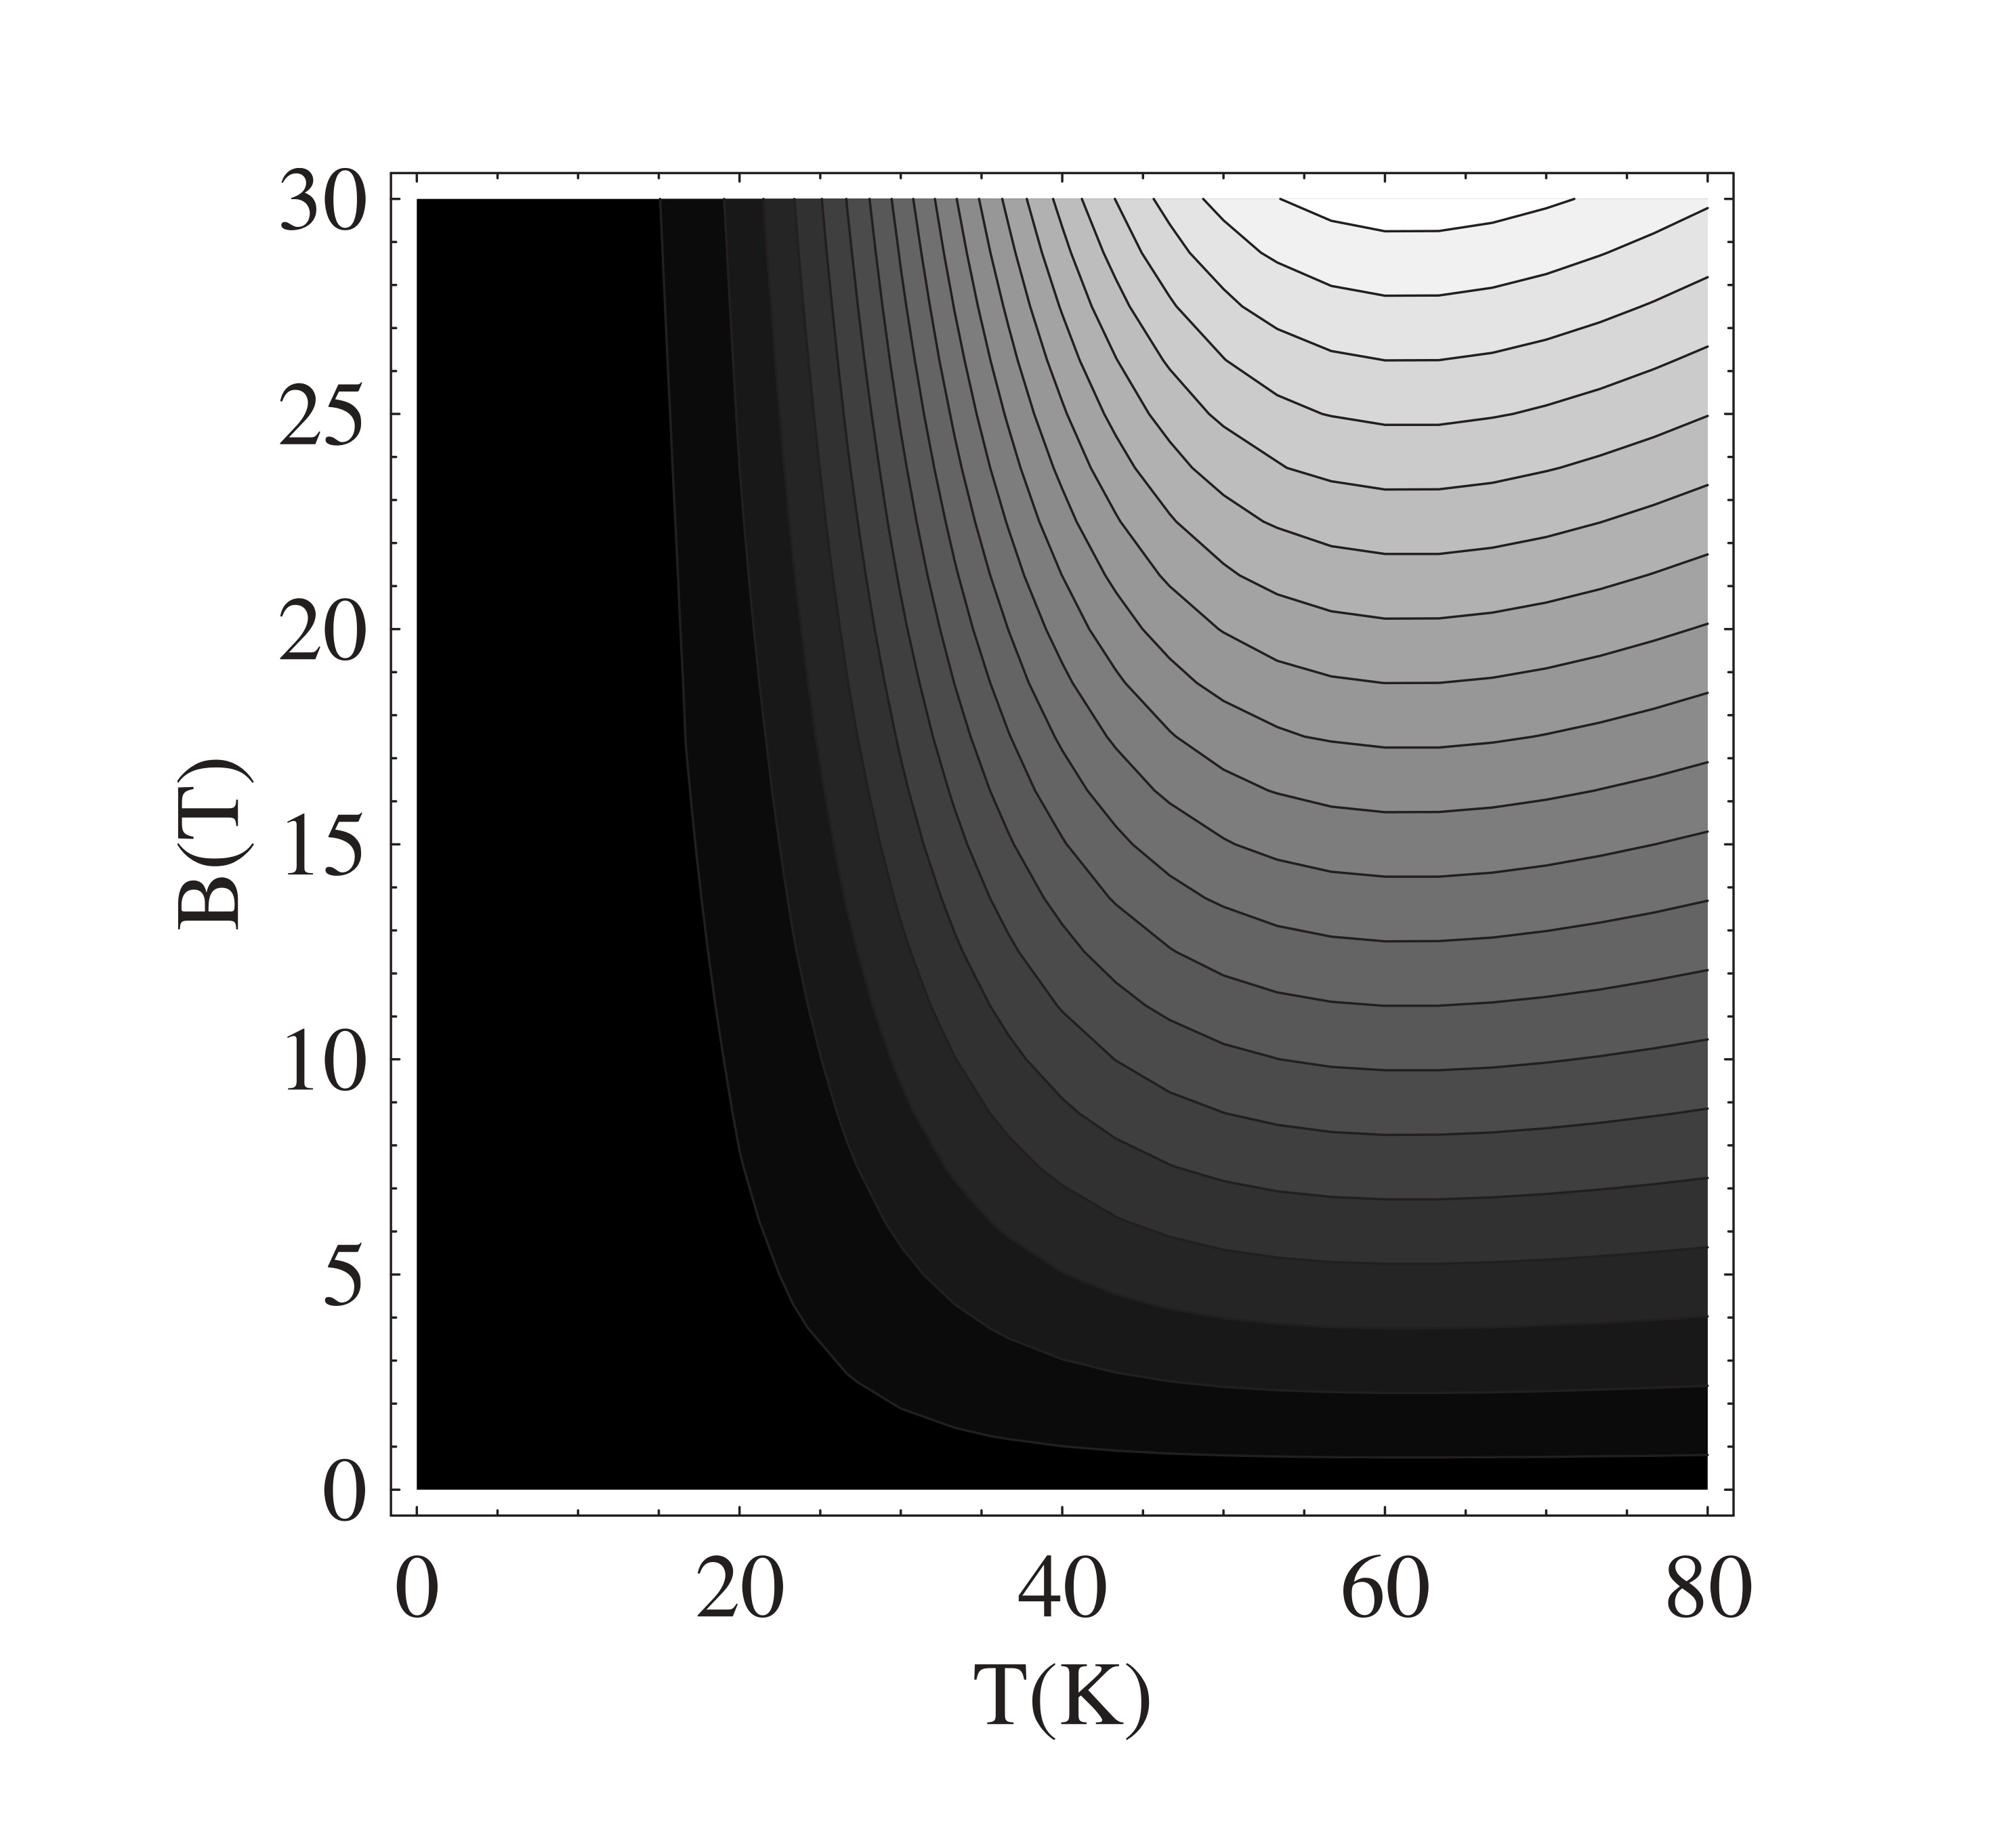
\includegraphics[scale=0.65]{eN.png}
						\caption{Estimated $e_N(B,T)$ for $x=0.12$ and $T>T_c\approx30K$. The strengh ranges up to $10\mathrm{\mu V/K}$. Extracted from {\scriptsize Hartnoll \textit{et al.}, PRB, \textbf{76}, 144502 (2007)}.}
					\end{figure}
				\end{column}
				\begin{column}{0.45\textwidth}
					\begin{figure}[!htp]
						\centering
						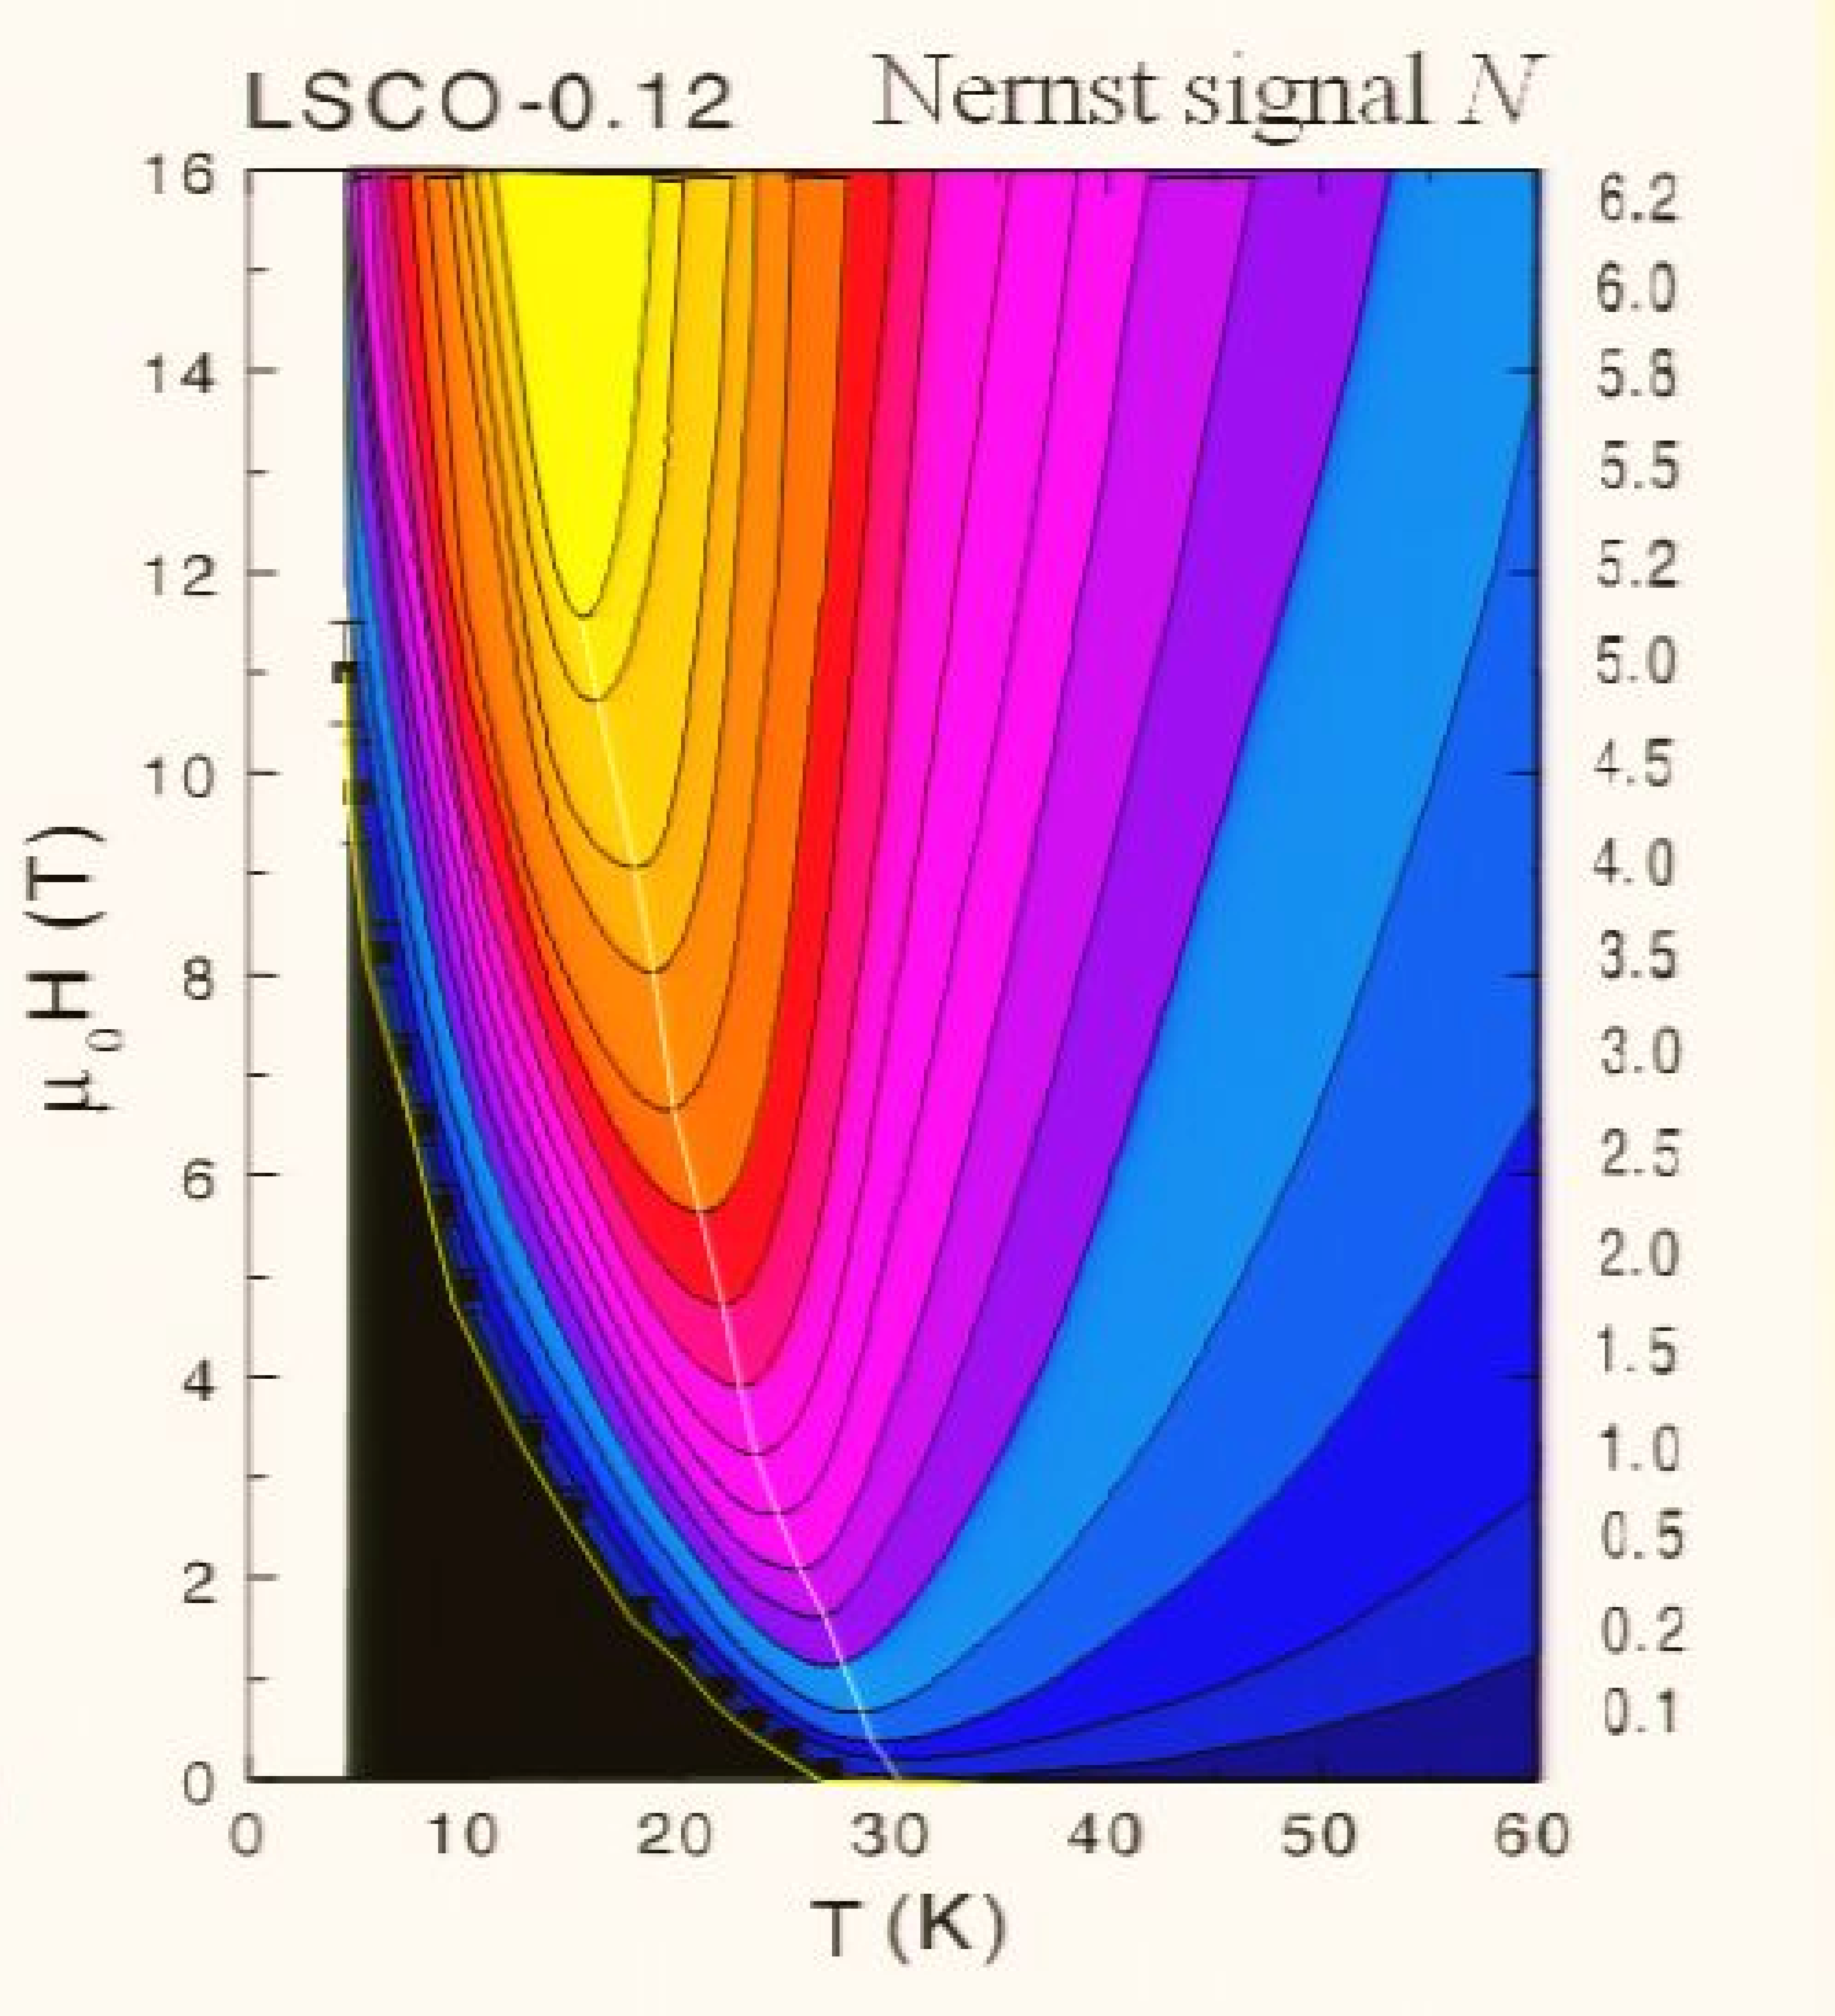
\includegraphics[scale=0.31]{Wang.png}
						\caption{Measured $e_N(B,T)$. Converted from Fig (7) of {\scriptsize Wang \textit{et al.}, PRB, \textbf{73}, 024510 (2006)}. The unit is also $\mathrm{\mu V/K}$.}
					\end{figure}
				\end{column}
			\end{columns}
		\end{frame}

		\begin{frame}\frametitle{The End?}
			\begin{figure}[!htp]
				\centering
				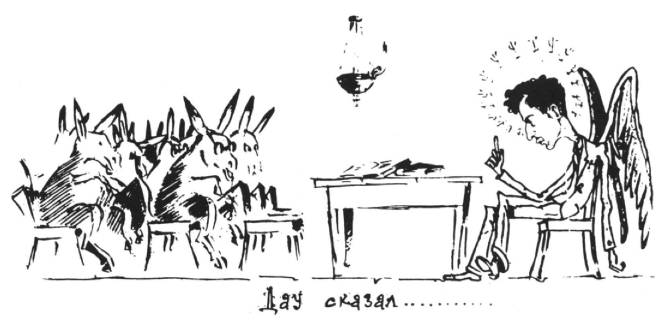
\includegraphics[scale=0.6]{Landau.png}
				\caption{When Landau teach his Jackass students about QM}
			\end{figure}
		\end{frame}

	\subsection{Negative Magnetoresistance in Weyl Semimetals: Anomalous Hydrodynamics}
		\begin{frame}\frametitle{Chiral Anomaly}
			\begin{block}{Anomaly}
				Anomaly is the phenomenon of the non-conservation of a classical symmetry in the quantum limit.
			\end{block}
			\only<2->{
			Consider applying $\bm{B}=B\hat{z}$ to the {\color{red}single} RH (3+1)-D Weyl fermion $H=\hbar v_F\bm{\sigma}\cdot\bm{p}$
			\begin{figure}[!htp]
				\centering
				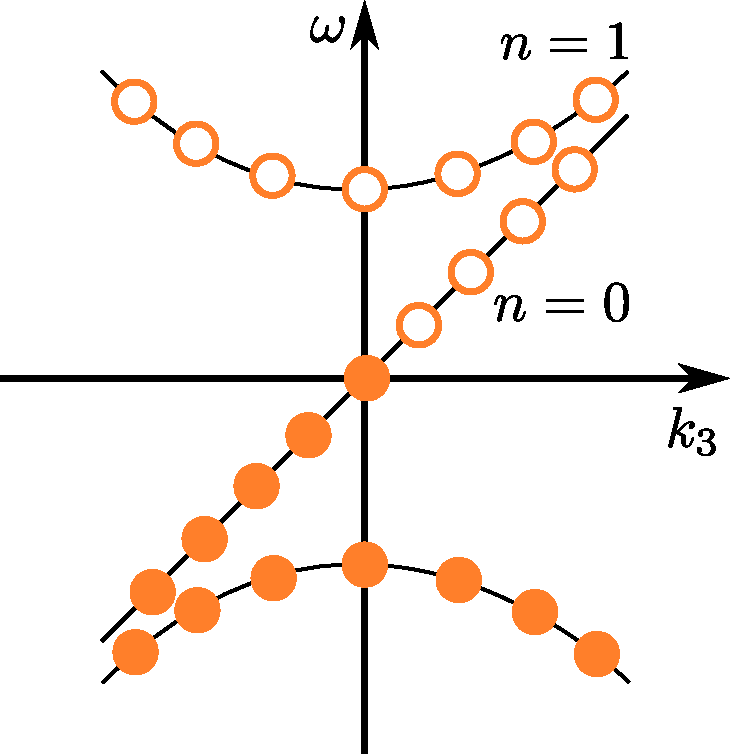
\includegraphics[scale=0.3]{Weyl-LL.pdf}
				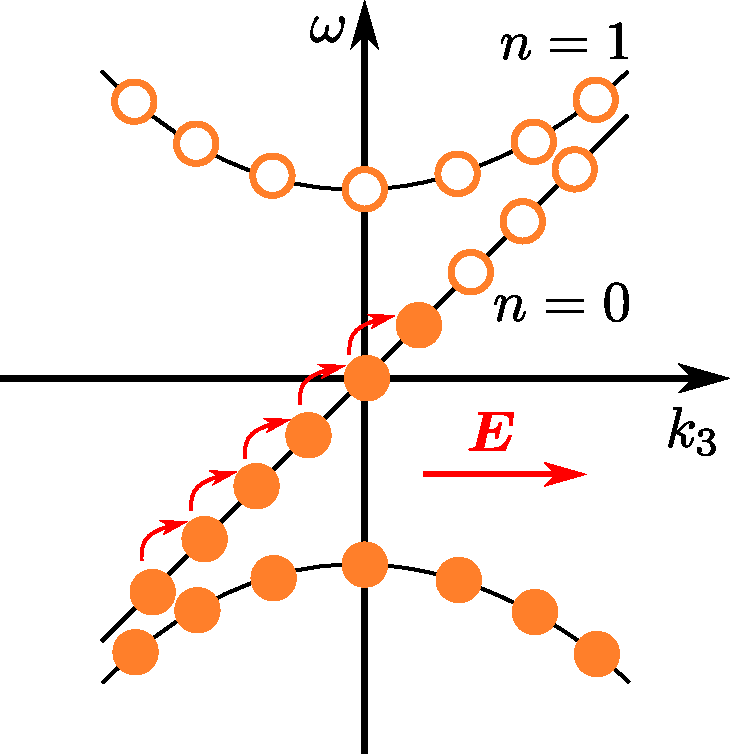
\includegraphics[scale=0.3]{Weyl-LL-2.pdf}
				\caption{Spectrum of Landau level when $\bm{E}\parallel\bm{B}$ is applied --- breakdown of charge conservation ({\scriptsize Nielsen\&Ninomiya, Phys. Lett. B, \textbf{130}, 6 (1983)})}
			\end{figure}
			}
		\end{frame}
		
		\begin{frame}\frametitle{Effects on Classical Hydrodynamics}
			When chiral anomaly is present, the equation of macroscopic charge conservation should be replaced by
			\begin{equation*}
				\partial_\mu \langle J^\mu\rangle=-\dfrac{C}{8}\varepsilon^{\mu\nu\rho\sigma}F_{\mu\nu}F_{\rho\sigma}=C\bm{E}\cdot\bm{B},\quad C=\dfrac{\pm1}{4\pi^2}.
			\end{equation*}
			\pause
			If we follow the previous steps working out the constitutive relation for $J^\mu$ and $T_{\mu\nu}$, a new row of data start to emerge due to the \textbf{\color{red}breakdown of parity-inversion symmetry} ({\scriptsize Bhattacharya \textit{et al.}, JHEP, \textbf{05}, 147 (2014)}).
			\only<2>{
				\begin{center}
					\begin{tabular}{c||c|c|c}
						& All Data & EOM & {\color{red}Independent Data}\\
						\hline\hline\\[-1em] %simple solution, see https://tex.stackexchange.com/questions/159257/increase-latex-table-row-height
						Pseudo- & $\omega^\mu\equiv\dfrac{1}{2}\varepsilon^{\mu\nu\alpha\beta}u_\nu \partial_\alpha u_\beta$ & & {\color{red}$\omega^\mu$}\\[1em]
						vectors & $B^\mu\equiv\dfrac{1}{2}\varepsilon^{\mu\nu\alpha\beta}u_\nu F_{\alpha\beta}$ & & {\color{red}$B^\mu$}
					\end{tabular}
				\end{center}
			}
			\only<3->{
				\\[1em]So after entropy production argument ({\scriptsize Son\&Sur\'{o}wka, PRL, \textbf{103}, 191601 (2009)})
				\begin{align*}
					J^\mu&=\rho u^\mu-\sigma_Q TP^{\mu\nu}\partial_\nu \left(\dfrac{\mu}{T}\right)+\sigma_Q E^\mu+{\color{red}\xi\omega^\mu+\xi_B B^\mu}\\
					\xi&=C \left(\mu^2-\dfrac{2}{3}\dfrac{\mu^3\rho}{\varepsilon+P}\right),\quad \xi_B=C \left(\mu-\dfrac{1}{2}\dfrac{\rho\mu^2}{\varepsilon+P}\right).
				\end{align*}
			}
		\end{frame}

		\begin{frame}\frametitle{Gravitational Anomaly}
			Motivated by Luttinger's pioneer work on thermal transport ({\scriptsize Luttinger, PR, \textbf{135}, A1505 (1964)}), {\color{red}thermal gradient can be brought in through the gravitation fields}. So a curved space with Riemann curvature $R_{\alpha\beta\mu\nu}$ should also be taken into account.\\[1em]
			\pause
			Using Fujikawa's (1979) technique, the full conservation laws are ({\scriptsize Alvarez-Gaumé\&Witten, Nuclear Phys. B, \textbf{234}, 2 (1984)})
			\begin{block}{Conservation Law}
				\begin{align*}
					\nabla_\mu J^\mu&=-\dfrac{C}{8}\varepsilon^{\mu\nu\rho\sigma}F^{\mu\nu}F^{\rho\sigma}-\dfrac{G}{32\pi^2}\varepsilon^{\mu\nu\rho\sigma}R^\alpha_{\beta\mu\nu}R^\beta_{\alpha\rho\sigma},\\
					\nabla_\mu T^{\mu\nu}&=F^{\nu\mu}J_\mu-\dfrac{G}{16\pi^2}\nabla_\mu\bigg(\varepsilon^{\rho\sigma\alpha\beta}F_{\rho\sigma}R_{\alpha\beta}^{\nu\mu}\bigg),\quad G=\dfrac{\pm1}{24}
				\end{align*}
				\textbf{\color{red}Coefficent $G$ is intrinsic that even in flat space (as is done in experiments), the charge current will displays some dependence on that!}
			\end{block}
		\end{frame}

		\begin{frame}\frametitle{Failure on Single Weyl Node}
			\begin{redblock}{Nielsen-Ninomiya Theorem  (1981)}
				Weyl nodes of distinct charality must come into pairs on an even-dimension lattice (due to periodicity) so that the net Berry flux vanishes.
			\end{redblock}
			\only<2-3>{Q: How to calculate the transport coefficients for system with multiple Weyl nodes?\\[1em]
			A naive guess is that we can obtain the transport properties for one chiral fluid, and then add them together to get the net conductivities.\only<3>{But \textbf{this is NOT TRUE} for periodic system since
			\begin{equation*}
				0=\int\dd^3\bm{x}\,\partial_\mu J^\mu{\color{red}\neq}\int\dd^3\bm{x}\,C\bm{E}\cdot\bm{B}.
			\end{equation*}}}
			\only<4->{
				On the lattice where Nielsen-Ninomiya theorem applies
				\begin{equation*}
					0=\int\dd^3\bm{x}\,\partial_\mu J^\mu_{\text{total}}{\color{red}=}\int\dd^3\bm{x}\,\bm{E}\cdot\bm{B}\sum_a C_a=0
				\end{equation*}
				\vspace{-2em} %useful for reducing blank space, see https://tex.stackexchange.com/questions/30062/vspace-vs-vskip
				\begin{columns}
					\begin{column}{0.45\textwidth}
						\begin{itemize}
							\item Expect balance for a finite DC conductivity: UV Physics of intervalley scattering ({\scriptsize Son\&Spivak, PRB, \textbf{88}, 104412 (2013)})
							\item Similar argument for the heat current $\partial_i Q^i_a=2G_aT\nabla T\cdot\bm{B}$.
						\end{itemize}
					\end{column}
					\begin{column}{0.5\textwidth}
						\begin{figure}[!htp]
							\centering
							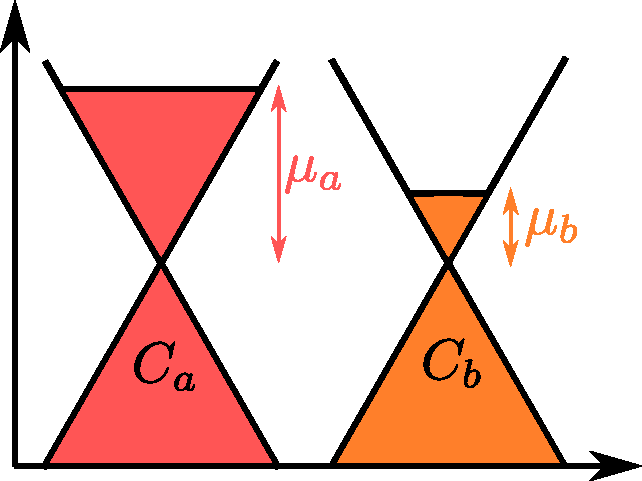
\includegraphics[scale=0.35]{Neilsen.pdf}
						\end{figure}
					\end{column}
				\end{columns}
			}
		\end{frame}
		
		\begin{frame}\frametitle{Hydrodynamic EOM with Intervalley Scattering}
			In the proper reference frame, the charge current has the form of ({\scriptsize Lucas \textit{et al.}, PNAS, \textbf{113}, 34 (2016)}) 
			\begin{align*}
				\bm{J}_a&=(\bm{J}_a)_{\text{non-chiral}}+\mathcal{D}_1\nabla\times\bm{v}+\dfrac{D_2}{2}\bm{B},\quad T^{\mu\nu}_a=(T^{\mu\nu}_a)_{\text{non-chiral}}.\only<1>{\\
				\mathcal{D}_1&=\dfrac{C\mu^2}{2}\left(1-\dfrac{2}{3}\dfrac{\rho\mu}{\varepsilon+P}\right)-\dfrac{4G\mu\rho T^2}{\varepsilon+P},\quad \mathcal{D}_2=C\mu \left(1-\dfrac{1}{2}\dfrac{\rho\mu}{\varepsilon+P}\right)-\dfrac{GT^2\rho}{\varepsilon+P}.}
			\end{align*}
			\only<2>{
			\vspace{1em}
			Q: How to incorporate all intervalley scattering processes?
			}
			\only<3->{
				\vspace{-1em}
				\begin{block}{Phenomenological Hydrodynanic EOM}
				\vspace{-1em}
					\begin{align*}
						\partial_\mu J^\mu_a&=-\sum_b\bigg(\mathcal{R}_{ab}\nu_b+\mathcal{S}_{ab}\beta_b\bigg)&\text{(charge)}\\
						\partial_\mu T^{\mu0}_a&=\sum_b\bigg(\mathcal{U}_{ab}\nu_b+\mathcal{V}_{ab}\beta_b\bigg)&\text{(energy)}
					\end{align*}

				\end{block}
				where $\nu_a\equiv \mu_a/T_a$, $\beta_a\equiv 1/T_a$, and
				\begin{equation*}
					\sum_b\mathcal{R}_{ab}=\sum_b\mathcal{S}_{ab}=\sum_b\mathcal{U}_{ab}=\sum_b\mathcal{V}_{ab}\equiv0.
				\end{equation*}

			}

		\end{frame}
		
		\begin{frame}\frametitle{Conductivity Matrix}
			After solving the linearized hydrodynamic EOM and reading out the conductivity (where $\bm{B}=B\hat{z}$), one gets ({\scriptsize Lucas \textit{et al.}, PNAS, \textbf{113}, 34 (2016)})
			\begin{equation*}
				\sigma_{ij}=\left(\begin{array}{ccc}
					\sum_a\dfrac{\rho_a^2\Gamma_a}{\Gamma_a^2+B^2\rho_a^2} & \sum_a\dfrac{\rho_a^3B}{\Gamma_a^2+B^2\rho_a^2}  & \\
					\sum_a\dfrac{-\rho_a^3B}{\Gamma_a^2+B^2\rho_a^2} & \sum_a\dfrac{\rho_a^2\Gamma_a}{\Gamma_a^2+B^2\rho_a^2} & \\
					& & \sum_a\dfrac{\rho_a^2}{\Gamma_a}+\mathfrak{s}B^2
				\end{array}\right),
			\end{equation*}
			where \textbf{$\Gamma_a$ represents the momentum relaxation rate} and
			\begin{equation*}
				\mathfrak{s}\equiv T \left(\begin{array}{cc}
					C_a & \mu C_a
				\end{array}\right)
				\left(\begin{array}{cc}
					\mathcal{R}_{ab} & \mathcal{-S}_{ab}\\
					\mathcal{-U}_{ab} & \mathcal{V}_{ab}
				\end{array}\right)^{-1}
				\left(\begin{array}{c}
					C_b\\ \mu C_b
				\end{array}\right) .
			\end{equation*}
			\only<2>{
				\vspace{-1em}
				\begin{redblock}{Drude Physics}
					\begin{equation*}
						\sigma=i\mathcal{D}/\pi(\omega+i\Gamma)
					\end{equation*}
				\end{redblock}
			}
			\only<3->{
			\vspace{-1em}
			\begin{redblock}{Electrical Negative Magnetoresistance}
				\begin{equation*}
					\sigma_{ij}\equiv\sigma_{ij}^{\text{Drude}}(B)+{\color{red}\mathfrak{s}B_i B_j}.
				\end{equation*}
			\end{redblock}
			}

		\end{frame}
		
		\begin{frame}\frametitle{Thermoelectric Response}
			\begin{redblock}{Thermalelectric Negative Magnetoresistance}
				\begin{equation*}
					\alpha_{ij}\equiv\alpha_{ij}^{\text{Drude}}+\mathfrak{a}B_iB_j,\quad \bar{\kappa}\equiv\bar{\kappa}_{ij}^{\text{Drude}}+\mathfrak{b}B_iB_j
				\end{equation*}
			\end{redblock}
			where
			\begin{align*}
				\mathfrak{a}&=2T^2\left(\begin{array}{c}
					0\\G_a
				\end{array}\right)^{-1}
				\left(\begin{array}{cc}
					\mathcal{R}_{ab} & \mathcal{-S}_{ab} \\
					\mathcal{-U}_{ab} & \mathcal{V}_{ab}
				\end{array}\right)^{-1}
				\left(\begin{array}{c}
					C_b \\ \mu C_b
				\end{array}\right),\\
				\mathfrak{b}&=4T^2\left(\begin{array}{c}
					0\\G_a
				\end{array}\right)^{-1}
				\left(\begin{array}{cc}
					\mathcal{R}_{ab} & \mathcal{-S}_{ab} \\
					\mathcal{-U}_{ab} & \mathcal{V}_{ab}
				\end{array}\right)^{-1}
				\left(\begin{array}{c}
					0 \\ G_b
				\end{array}\right).
			\end{align*}
			\only<2->{All anomalous terms for $\alpha_{ij}$ and $\bar{\kappa}_{ij}$ vanish if $G_a=0$. So \textbf{\color{red}observation of thermolelectric negative magneotoresistance is a manifestation of gravitational anomaly!}
			}
		\end{frame}
		
		\begin{frame}\frametitle{Experimental Results}
			\only<1>{
				\begin{figure}[!htp]
					\centering
					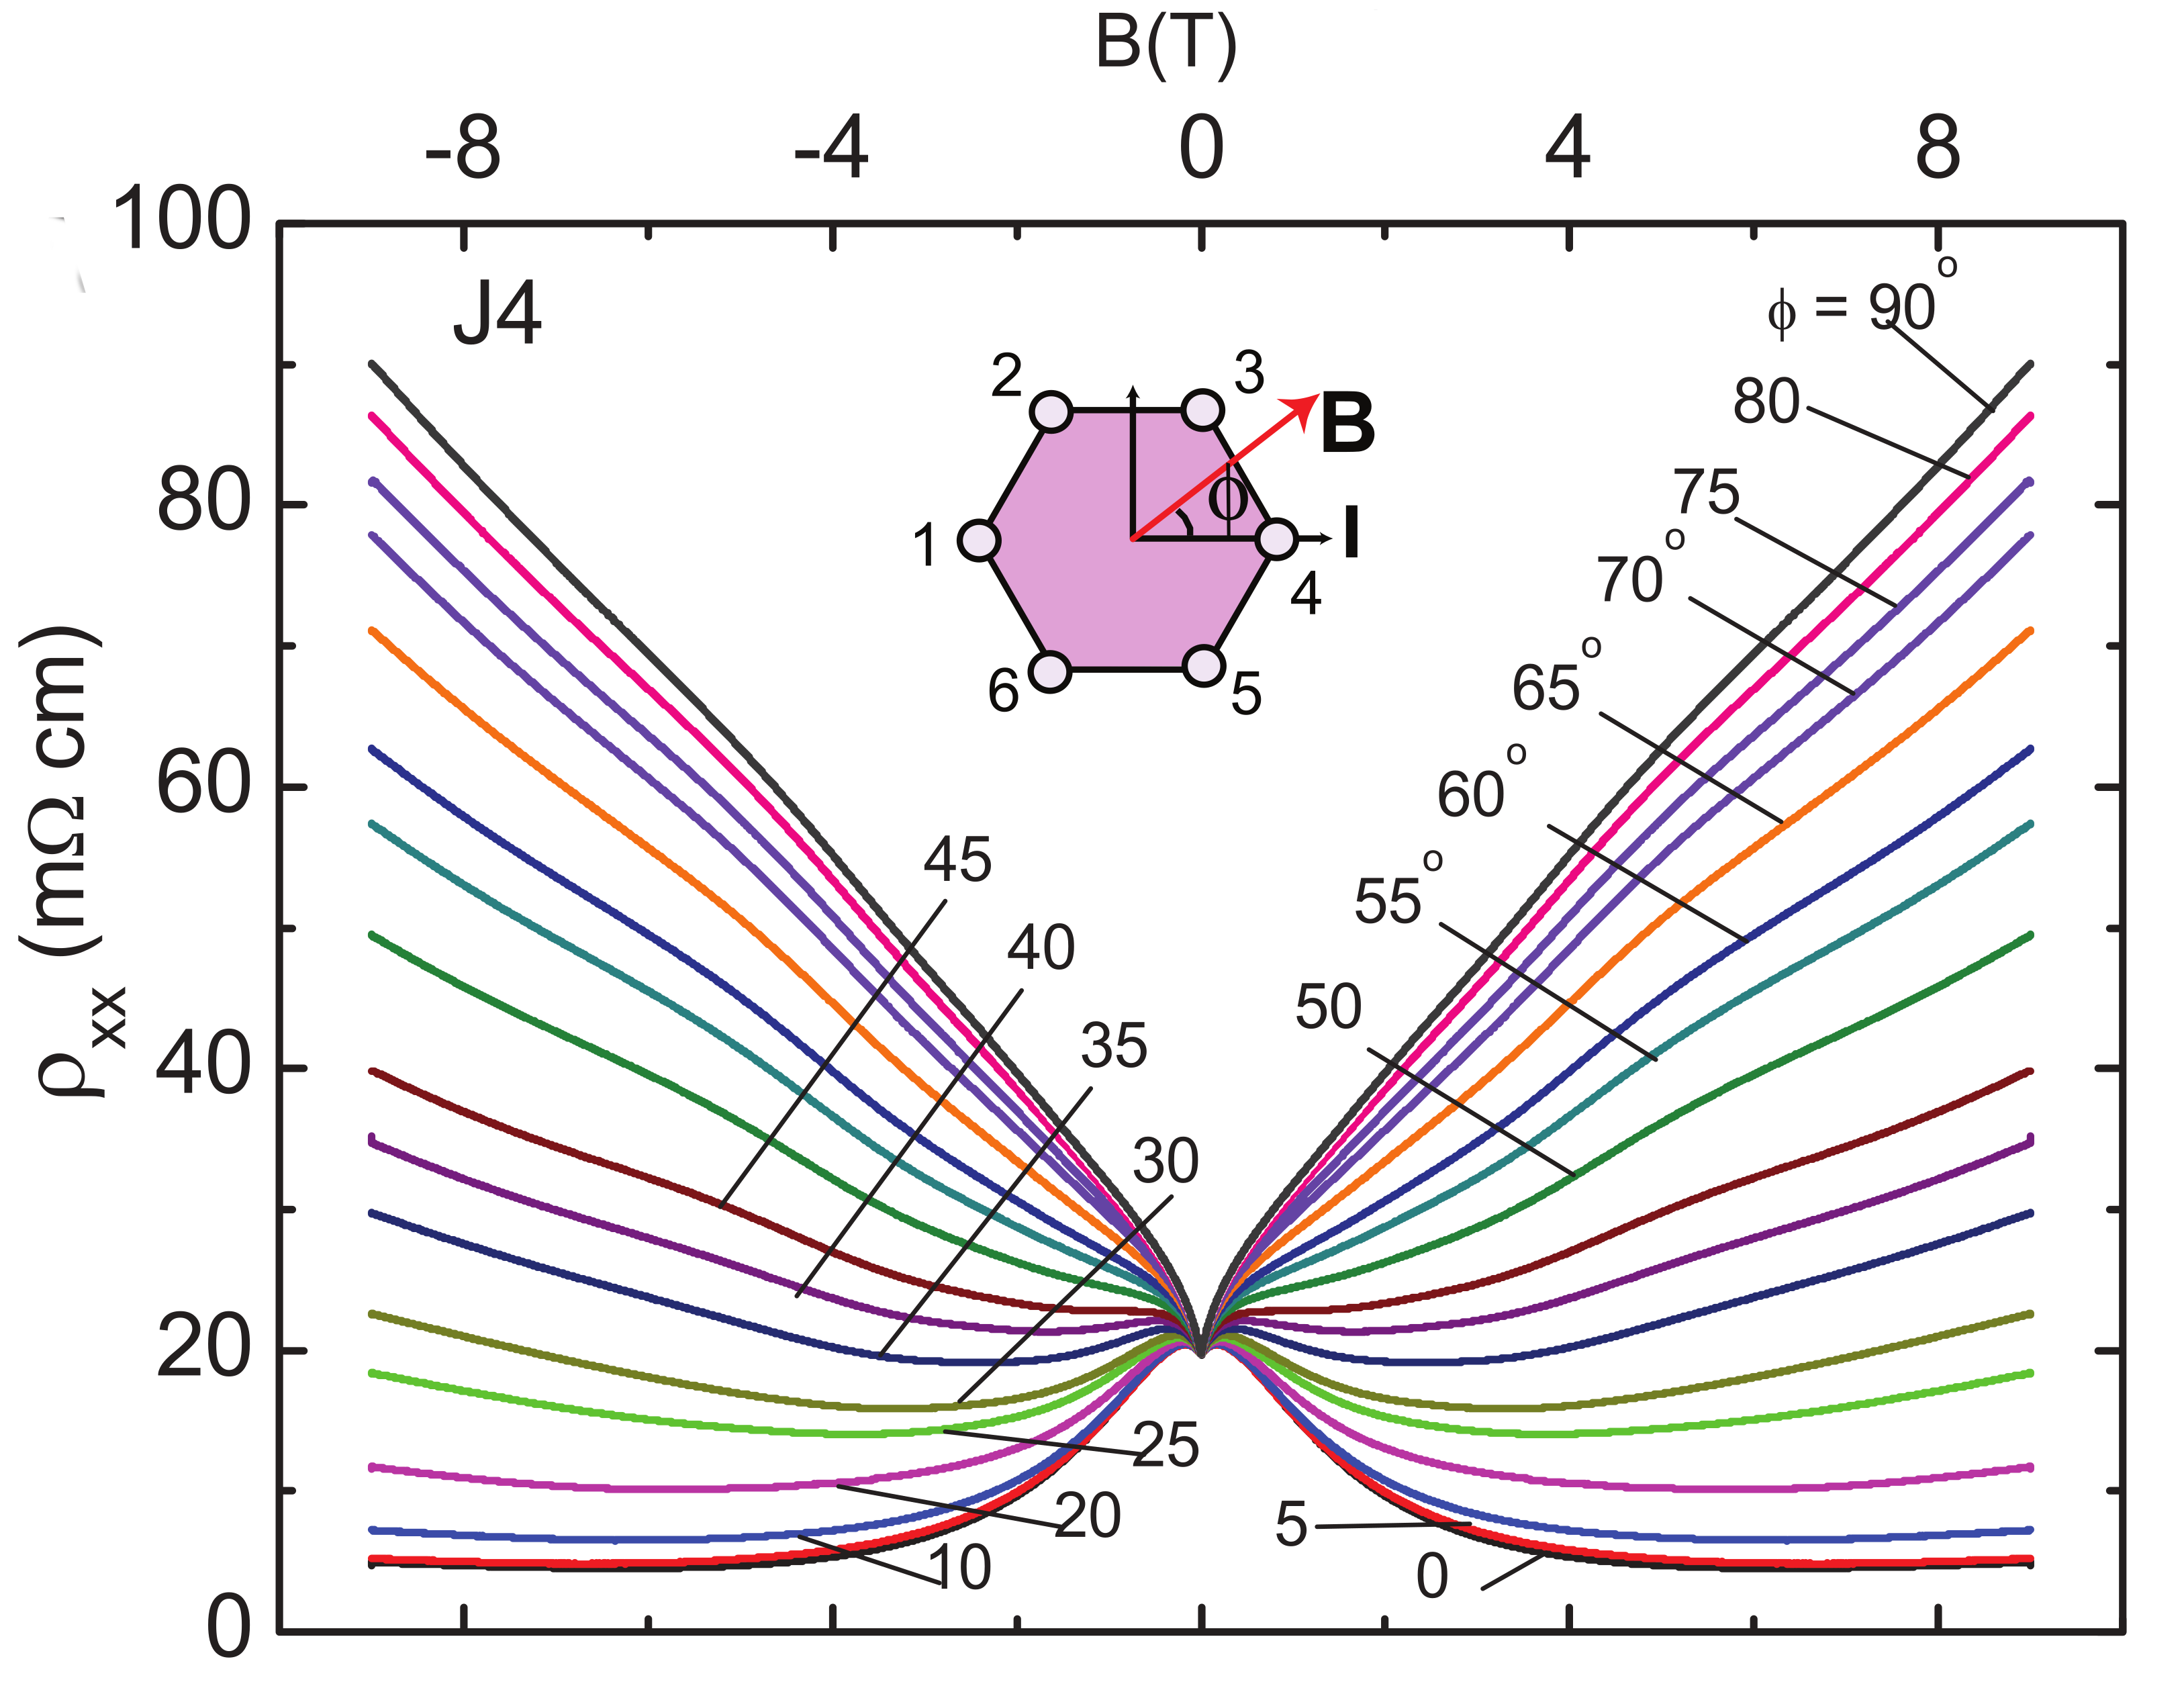
\includegraphics[scale=0.9]{Xiong.png}
					\caption{Evidence for the axial current in $\mathrm{Na_3Bi}$. Extraced from {\scriptsize Xiong \textit{et al}., Science, \textbf{350}, 6259 (2015)}.}
				\end{figure}
			}
			\only<2->{
				\begin{figure}[!htp]
					\centering
					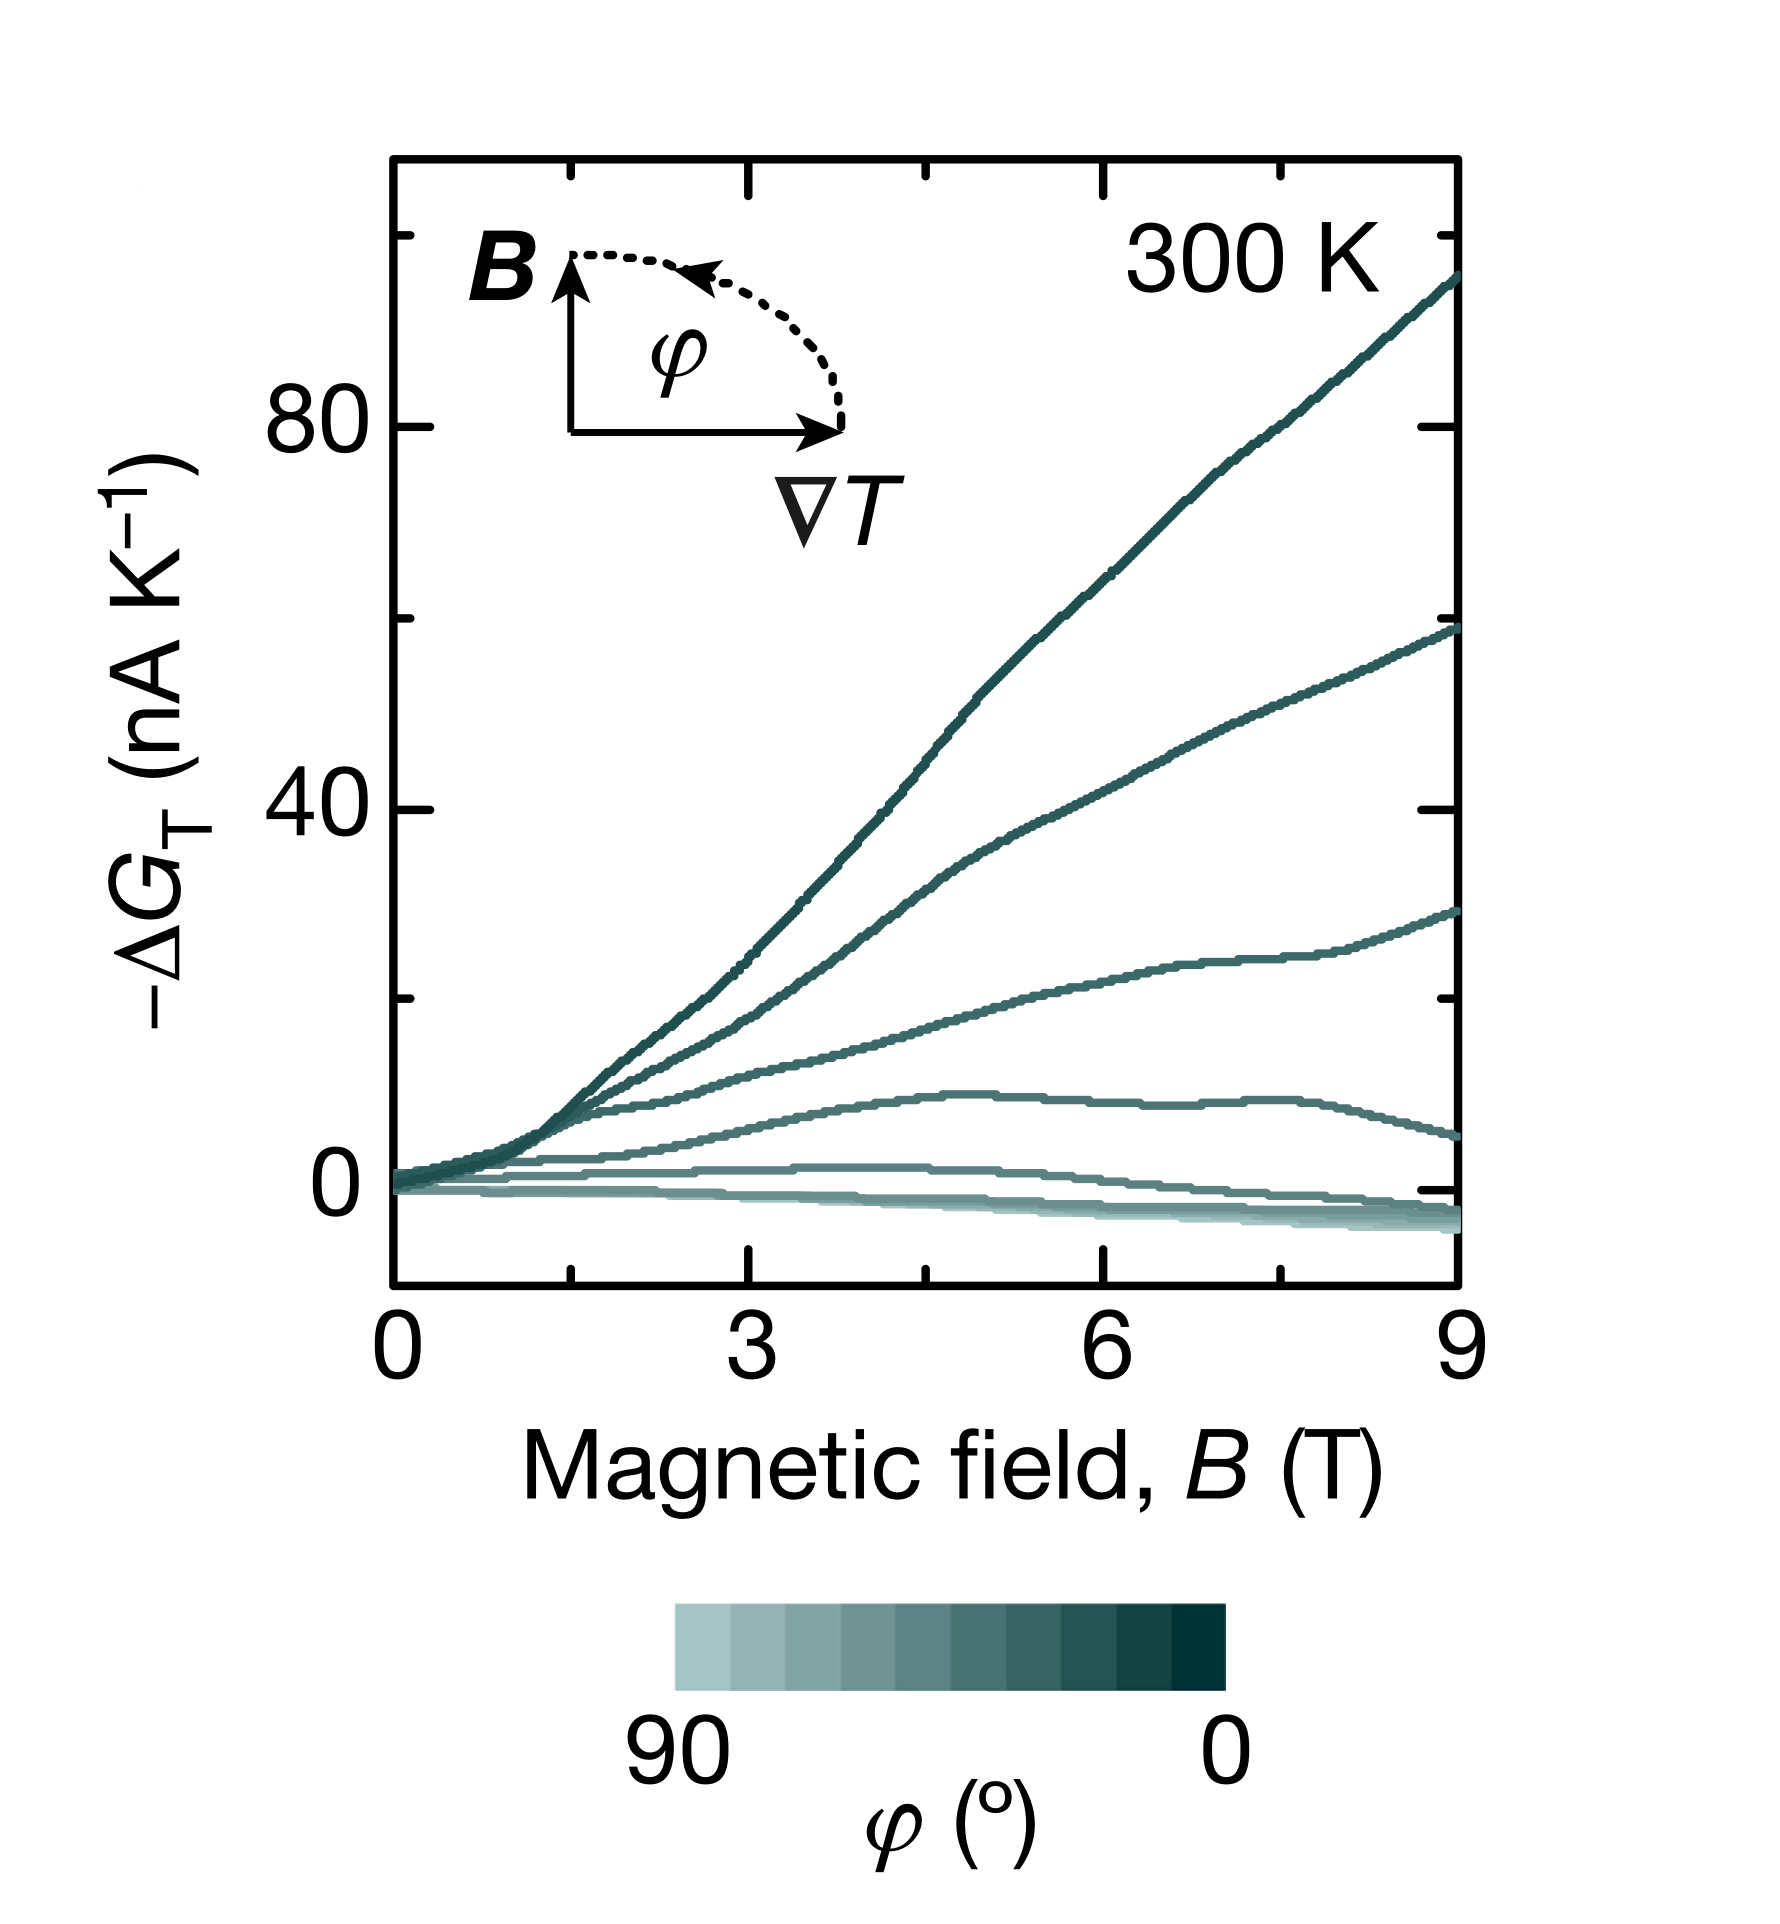
\includegraphics[scale=1.2]{Gooth.png}
					\caption{Evidence for the axial-gravitational anomaly in $\mathrm{NbP}$. Extracted from {\scriptsize Gooth \textit{et al.}, Nature, \textbf{547}, 7663 (2017)}.}
				\end{figure}
				
			}
		\end{frame}
		

%\section{Memory Matrix Formalism: Magnetotransport}

\section{Future Direction}
	\subsection{The Missing Piece}
		\begin{frame}\frametitle{Failure of Landau's Paradigm}
			\vspace{-1.5em}
			\begin{columns}
				\begin{column}{0.35\textwidth}
					\begin{figure}[!htp]
						\centering
						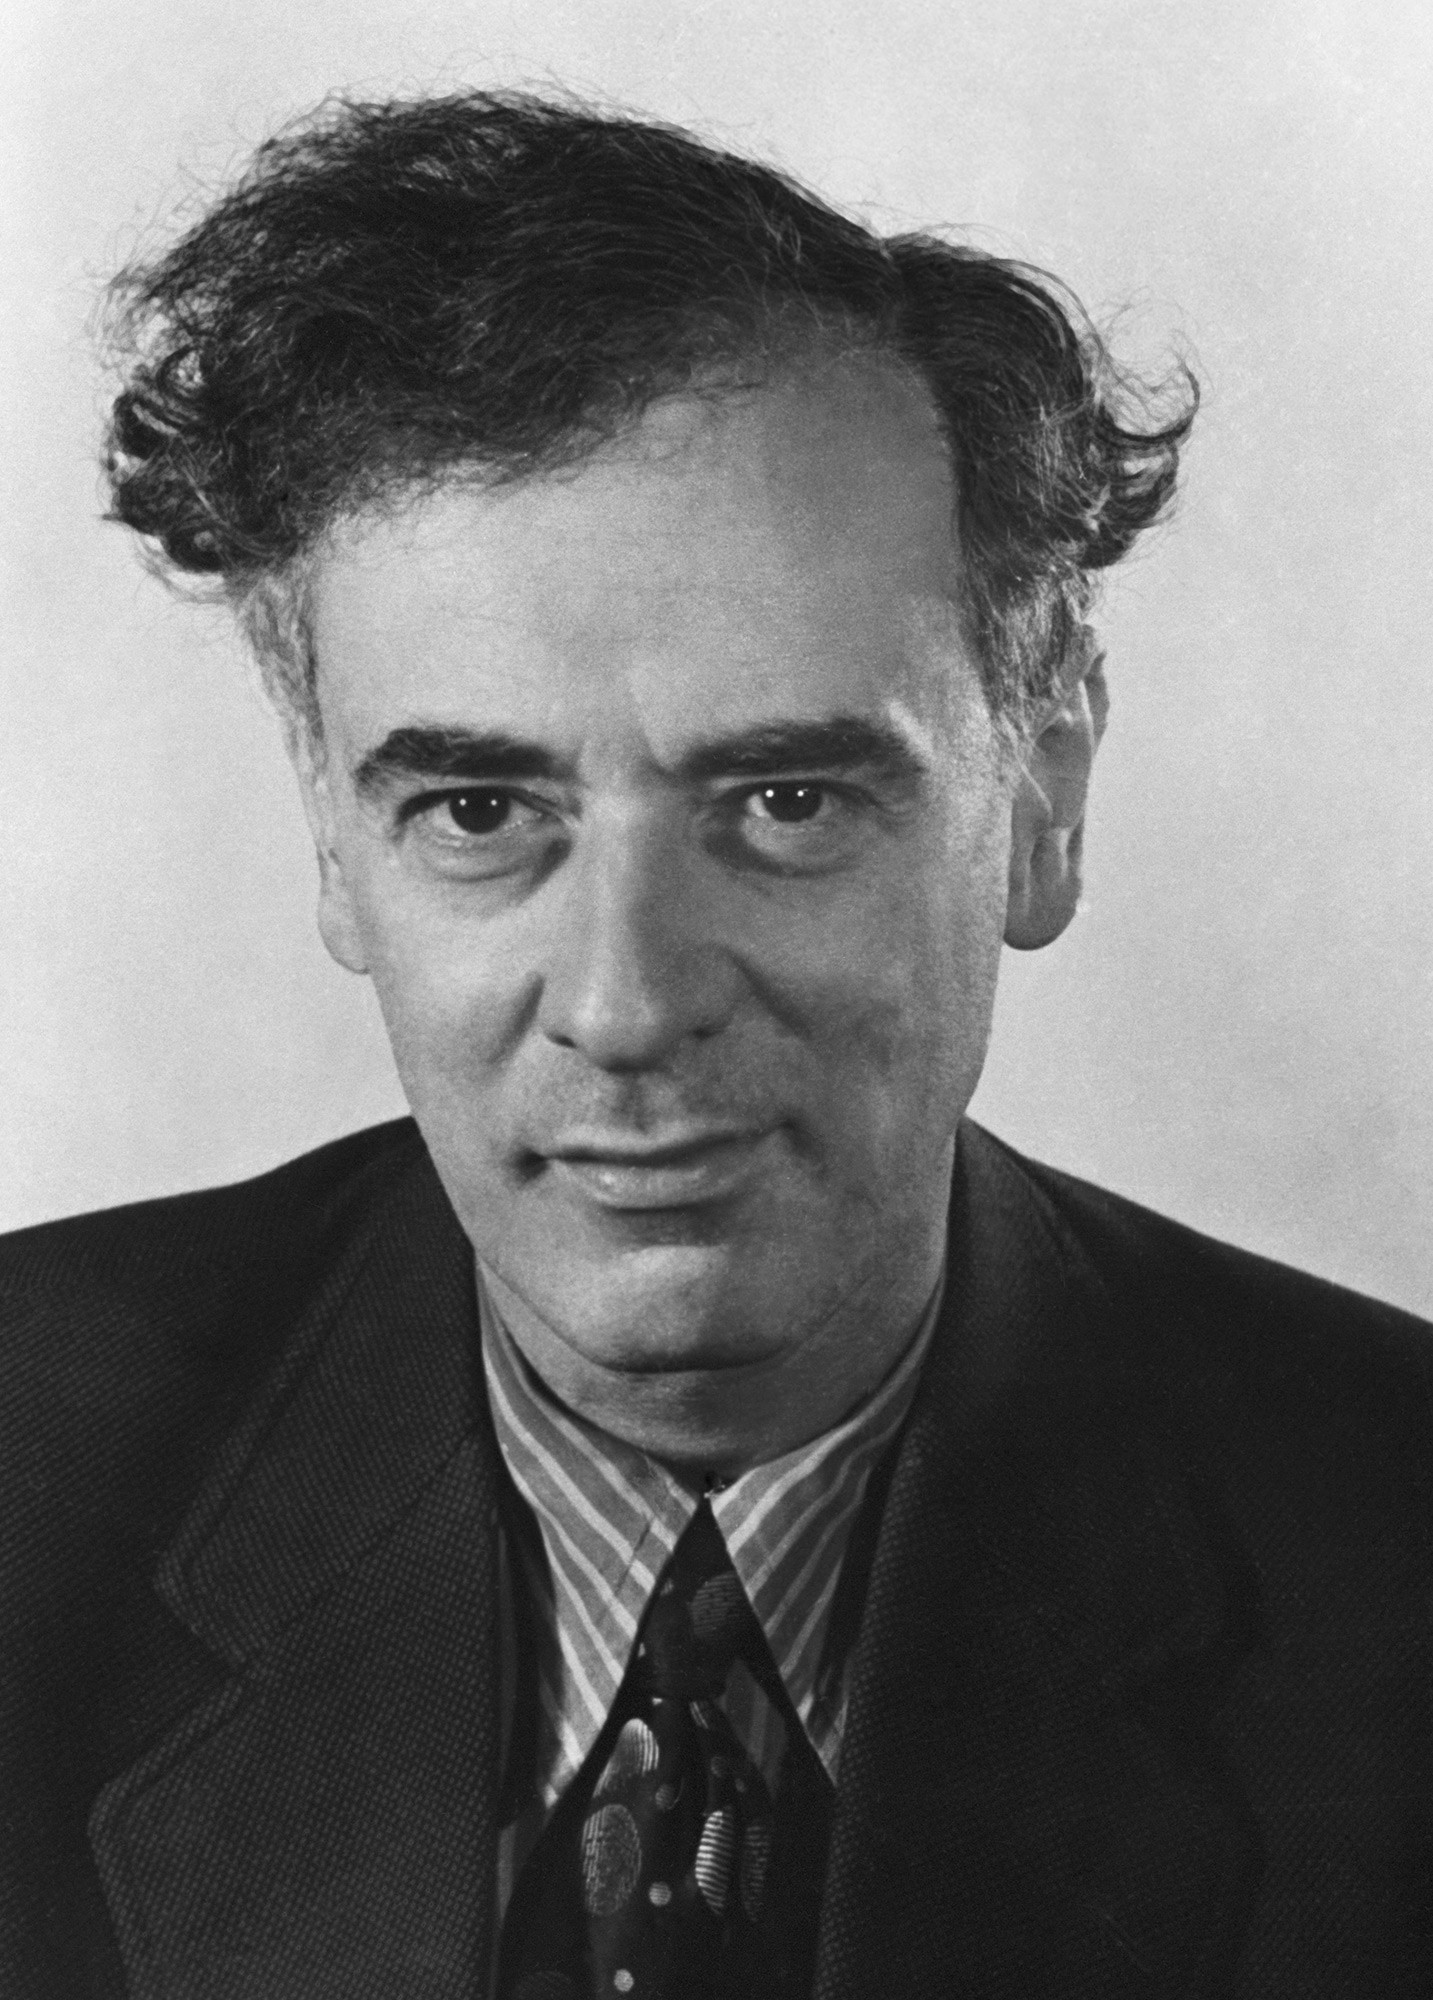
\includegraphics[scale=0.06]{Landau.jpg}
					\end{figure}
				\end{column}
				\begin{column}{0.6\textwidth}
					\begin{itemize}
						\item \textbf{Landau's Fermi Liquid Theory}
						\begin{itemize}
							\item Quasiparticle with mass etc. dressed by interactions;
							\item One-to-one correspondence between Fermi liquid and Fermi gas;
						\end{itemize}
						\item \textbf{Ginzberg-Landau Theory}
						\begin{itemize}
							\item Contiuous phase transition occurs only when symmetry is broken; 
							\item Field theory of continuous phase transition is described by the order parameter;
							\item Phases are classified by their symmetries.
						\end{itemize}
					\end{itemize}
				\end{column}
			\end{columns}
			\only<2->{
			\vspace{1em}
			\begin{columns}
				\begin{column}{0.5\textwidth}
					\textbf{SPT}: Haldane Chain, IQHE, TI, etc.
					\begin{itemize}
						\item Protected by symmetry
						\item Anomalous edges
						\item No topological order
						\item Short-range entanglement
					\end{itemize}
				\end{column}
				\begin{column}{0.45\textwidth}
					\textbf{SET}: Spin Liquids, FQHE, etc
					\begin{itemize}
						\item Topological ordered
						\item Bulk anyonic exicitation
						\item Long-range entanglement
					\end{itemize}
				\end{column}
			\end{columns}
			}
		\end{frame}
		
		\begin{frame}\frametitle{Intrinsic Anomlous Hall Effect}
			\begin{figure}[!htp]
				\centering
				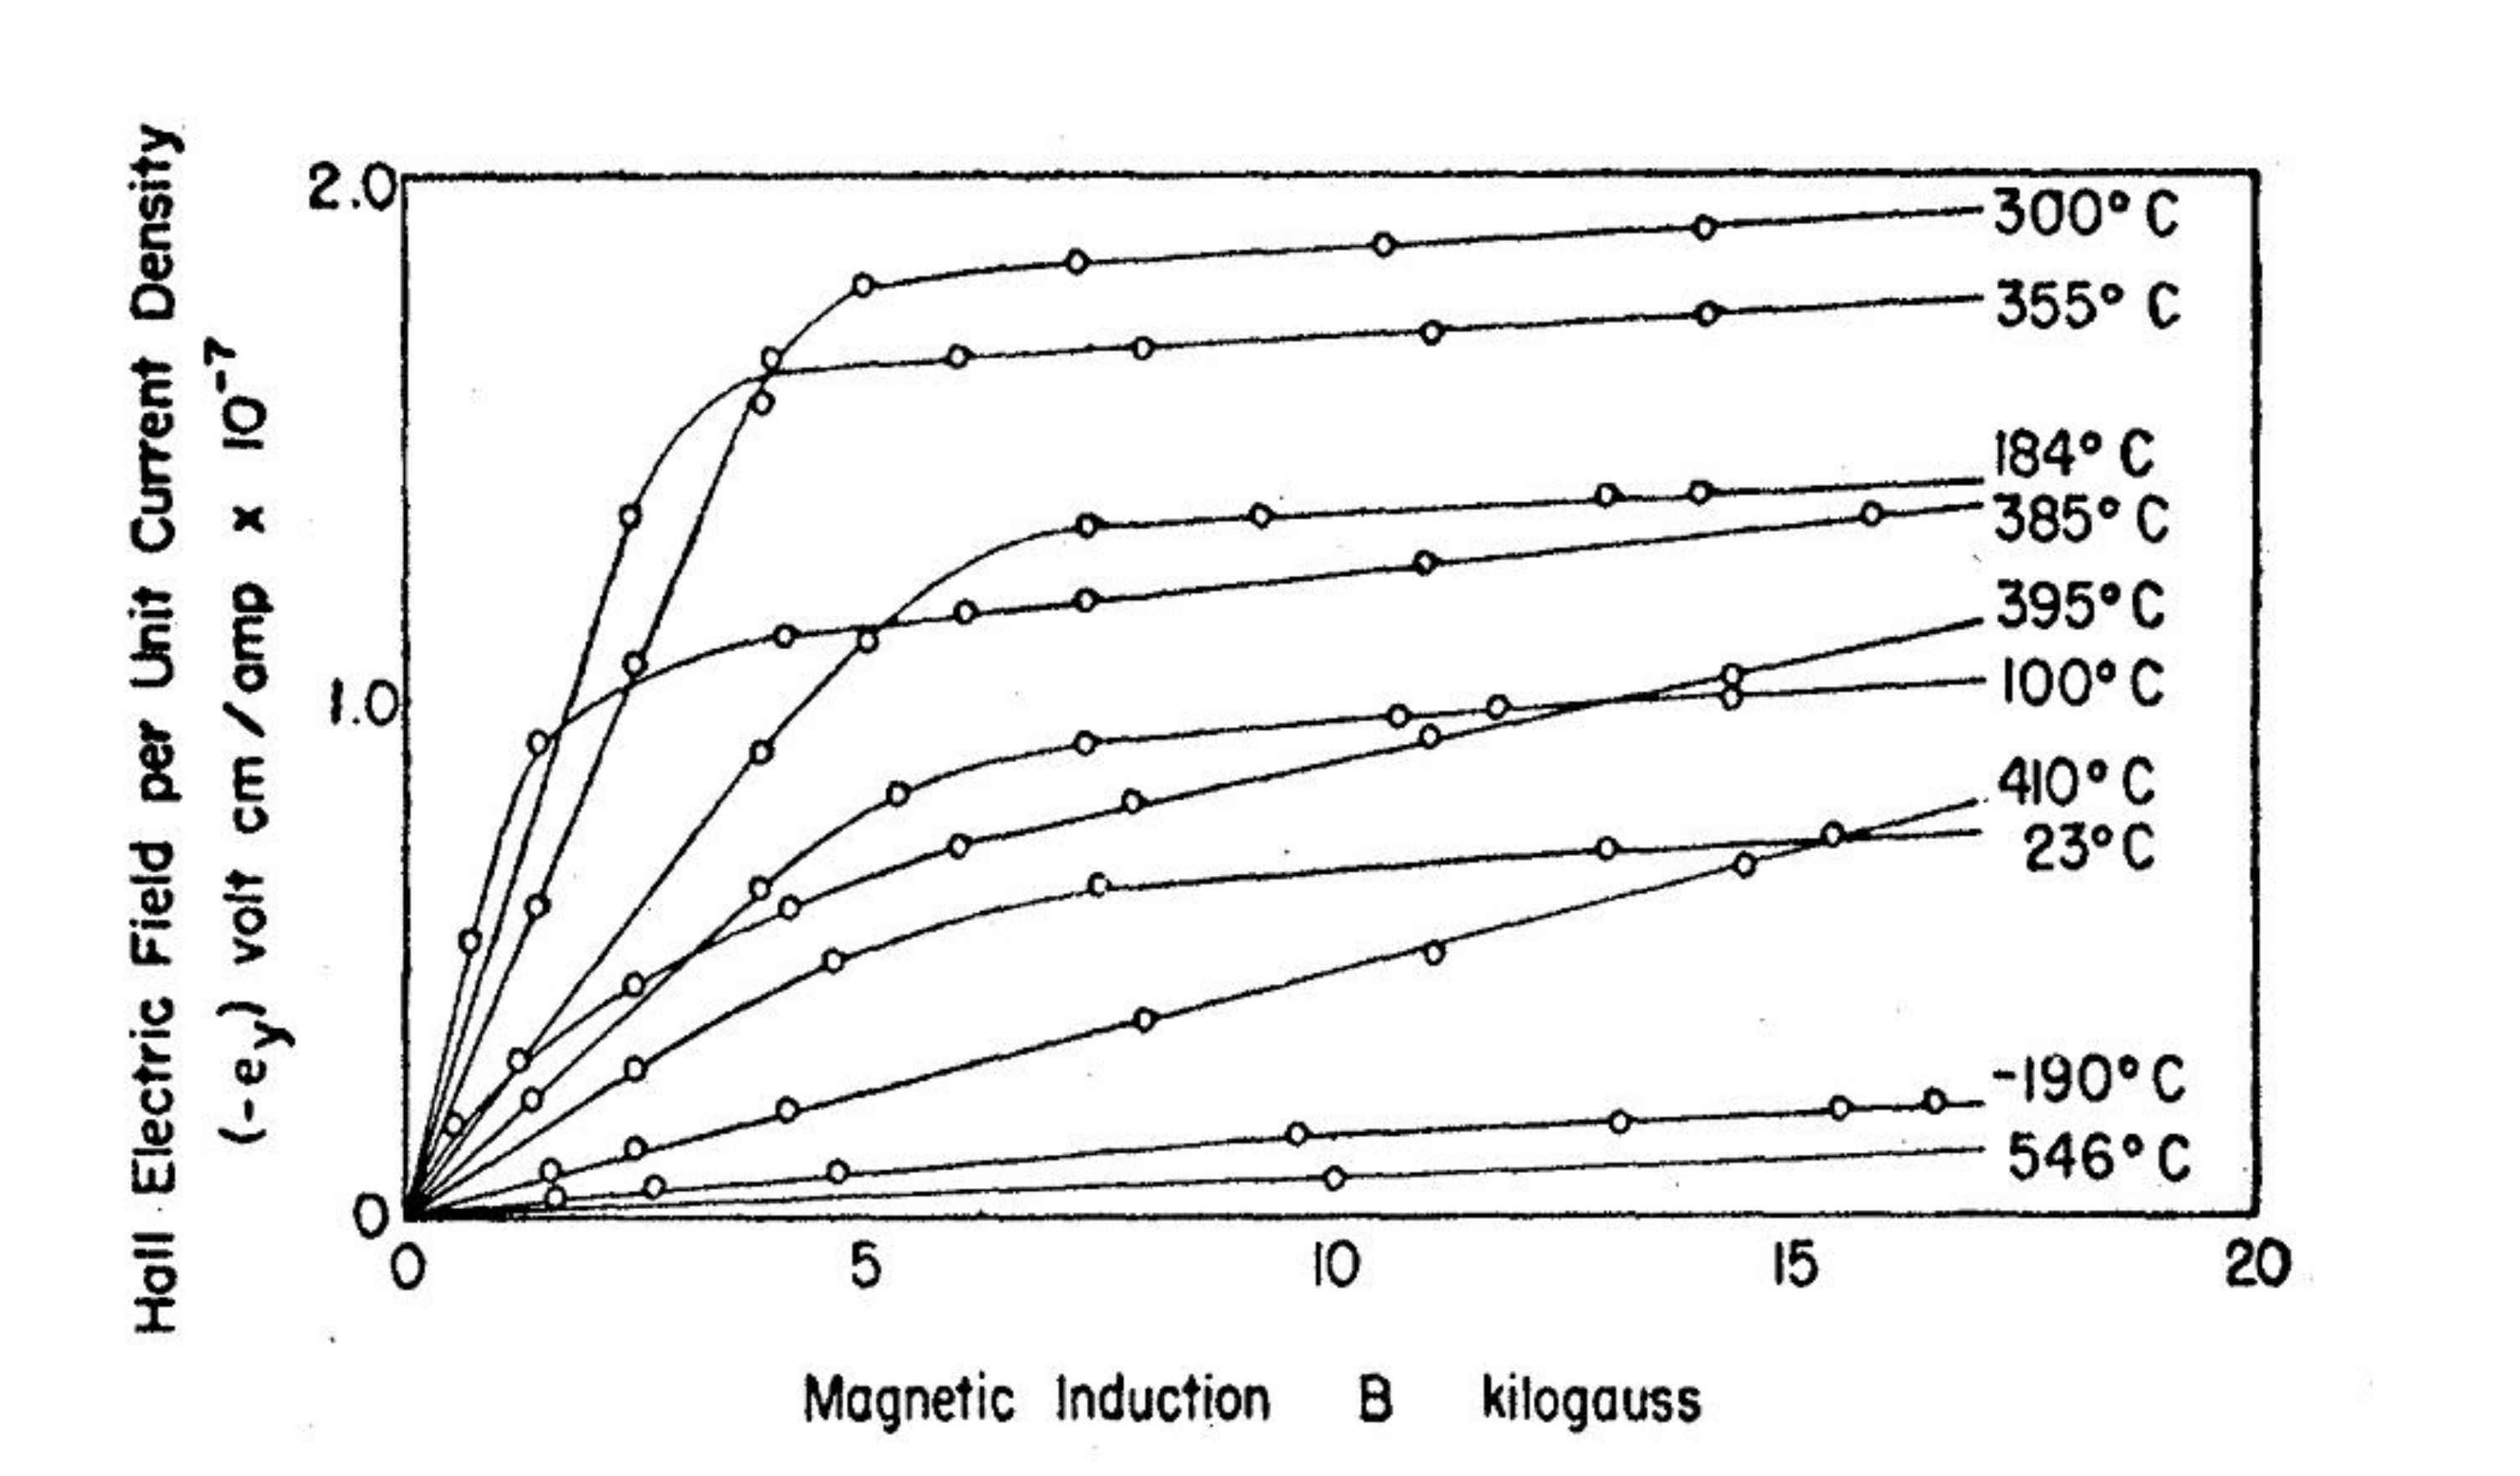
\includegraphics[scale=0.8]{AnomalousHall.png}
				\caption{Saturate dependence of Hall Resistivity on the perpendicular magnetic field. Extracted from {\scriptsize Paugh\&Rostoker, RMP, \textbf{25}, 151 (1953)}}
			\end{figure}
			\vspace{-1em}
			\pause
			Following KL theory ({\scriptsize Karplus\&Luttinger, PR, \textbf{95}, 5 (1954)}) where anomalous group velocity is introduced due to SOC, the topological nature of AHE was revealed ({\scriptsize Haldane, PRL, \textbf{93}, 206602 (2004)}) that
			\begin{block}{}
				\begin{equation*}
					\sigma^{ab}_0(\mu)=\dfrac{e^2}{\hbar}\dfrac{1}{\Omega N}\sum_{\bm{k}n}\mathcal{F}^{ab}_n f_n^0(\bm{k},\mu).
				\end{equation*}
			\end{block}
		\end{frame}
		
		\begin{frame}\frametitle{AHE in Weyl Semimetal}
			\begin{itemize}
				\item All transverse transport coefficient of Hydrodynamic theory with anomalies vanish when $B\rightarrow0$
				\begin{equation*}
					\sigma_{xy}=\sum_a\dfrac{B\rho_a^3}{\Gamma_a^2+B^2\rho_a^2},\quad \alpha_{xy}=\sum_a\dfrac{B\rho_a^2s_a}{\Gamma_a^2+B^2\rho_a^2},\quad \bar{\kappa}_{xy}=\sum_a\dfrac{BT\rho_a s_a^2}{\Gamma_a^2+B^2\rho_a^2}.
				\end{equation*}
				\pause
				\item But in principle, ther would be non-vanishing AHE in Weyl semimetal if the symmetry of Weyl nodes are low ({\scriptsize Yang, Lu, and Ran, PRB, \textbf{84}, 075129 (2011)})
				\begin{equation*}
					\sigma_{ij}=\dfrac{e^2}{2\pi\hbar}\varepsilon_{ijk}\nu_k,\quad \bm{\nu}=\sum_i (-1)^{\pm1}\bm{p}_i.
				\end{equation*}
			\end{itemize}
			\pause {\color{red}So there must be some intrinsic topological terms we missed in the hydrodynamic EOM (even with anomalies)!}
		\end{frame}
		
		
		
	\subsection{Future Direction}
		\begin{frame}\frametitle{Further Steps}
			\begin{itemize}
				\item Guessing the missing term in general hydrodynamic EOM (without relativistic structure).
				\item Obtaining the topological correction to all thermoelectric coefficients.
				\item Going to nonlinear level to derive more transport properties, and comparing with the non-trivial reciprocal relation founded by Xu and Ran (to be published)
				\begin{equation*}
					\dfrac{\partial \sigma_{ab}}{\partial A_c}+\dfrac{\partial \sigma_{bc}}{\partial A_a}+\dfrac{\partial \sigma_{ca}}{\partial A_b}\equiv0, \quad a,b,c \text{ stands for eletrical or thermal}.
				\end{equation*}
				\item Studying more realistic experiments with lower lattice symmetries (more terms will emerge).
				\item Finding out the origin of such topological term.
				\item $\cdots$
			\end{itemize}
		\end{frame}
		
		
	
\section*{Acknowlegement}
	\begin{frame}\frametitle{Acknowlegement}
		\textbf{Advisor}: Ying Ran\\
		\textbf{Collaborator}: Xu Yang\\
		\textbf{Committee Member}: Fazel Tafti, Xiao Chen\\[2em]

		\only<2>{
			\begin{center}
				\Huge Thanks!
			\end{center}
		}
	\end{frame}


\end{document}